%% Based on Omar Pardo's Thesis repository at Github (@opardo)
%% Based on a TeXnicCenter-Template by Tino Weinkauf.
%%%%%%%%%%%%%%%%%%%%%%%%%%%%%%%%%%%%%%%%%%%%%%%%%%%%%%%%%%%%%

%%%%%%%%%%%%%%%%%%%%%%%%%%%%%%%%%%%%%%%%%%%%%%%%%%%%%%%%%%%%%
%%% LATEX %%%
%%%%%%%%%%%%%%%%%%%%%%%%%%%%%%%%%%%%%%%%%%%%%%%%%%%%%%%%%%%%%
\documentclass[oneside,10pt,review,usenames,dvipsnames]{book}

%% Generales %%
%\usepackage[letterpaper, paperwidth=17cm, paperheight=22.5cm, top = 2cm, bottom = 1cm, inner = 1.5cm, outer = 1.5cm]{geometry}
\usepackage[paperwidth=17cm, paperheight=22.5cm, top = 2cm, bottom = 1cm, inner = 1.75cm, outer = 1.75cm]{geometry}
\usepackage[doublespacing]{setspace}
\usepackage[bottom]{footmisc}
\usepackage{enumerate}
\usepackage{fancyhdr} 
\usepackage{bm}
\usepackage{url}
\usepackage[usenames,dvipsnames]{xcolor}
            
%% Español y letras %%
\usepackage[spanish,es-nodecimaldot]{babel} 
\usepackage[utf8]{inputenc}
%\usepackage{lmodern} %Type1-font for non-english texts and characters
%\usepackage[T1]{fontenc}
%\usepackage{dsfont}

%% Tablas %%
\usepackage{longtable} 
\usepackage{multirow}
\usepackage{arydshln}
\usepackage{rotating}

%% Figuras %%
\usepackage{graphicx}
\usepackage{subcaption}
\usepackage{float}
\usepackage[font=scriptsize,labelfont=bf]{caption} 

%% Bibliografía %%
\usepackage[nottoc]{tocbibind}
\usepackage[backend=biber,style=chicago-authordate, natbib=true,ibidtracker = strict, opcittracker = strict]{biblatex}
\renewcommand*{\revsdnamedelim}{} %Se necesita para eliminar la coma antes de la conjunción "y" en una lista de dos nombres cuando el primero está  invertido (apellido, nombre)
\addbibresource{referencias_tesis_ACT.bib}
\addbibresource{referencias_tesis_RRII.bib}

%% Matemáticas %%
\usepackage{amsmath,amssymb,amsthm}
\usepackage[spanish,onelanguage,linesnumbered,ruled]{algorithm2e} %Algoritmos
\usepackage{mathtools} %Mejoras a símbolos matemáticos (y shortintertext)

%% Corrección espacios %%
\allowdisplaybreaks
	\setlength\abovedisplayskip{-10pt plus 0 pt minus 0pt}
	\setlength\belowdisplayskip{-10pt plus 0 pt minus 0pt}
	\setlength{\abovedisplayshortskip}{-10pt plus 0 pt minus 0pt}
	\setlength{\belowdisplayshortskip}{-10pt plus 0 pt minus 0pt}

%% Nuevos nombres capítulos español %%
\addto\captionsspanish{%
  \renewcommand{\appendixname}{Anexo}
}
\addto\extrasspanish{%
\def\chapterautorefname{Capítulo}%
\def\appendixautorefname{Anexo}
}

%% Nuevos comandos mates %%

\renewcommand{\Pr}{\ensuremath{\mathbb{P}}}
\newcommand{\E}[1]{\ensuremath{\mathbb{E}\left[ #1 \right]}}
\renewcommand{\proofname}{Demostración}


\newtheorem{teo}{Teorema}[chapter] 
\newtheorem{cor}[teo]{Corolario}
\newtheorem{lem}[teo]{Lema}

\theoremstyle{definition}
	\newtheorem{axiom}{Axioma}
	\newtheorem{pos}[axiom]{Postulado}
	\newtheorem{dfn}{Definición}[chapter]
	\newtheorem*{dfn*}{Definición}
	\newtheorem{obs}{Observación}[chapter]
	\newtheorem*{obs*}{Observación}
	\newtheorem{propiedad}{Propiedad}
	\newtheorem*{propiedad*}{Propiedad}

%% Contenido (ToC) %%
\setcounter{tocdepth}{3}
\setcounter{secnumdepth}{3}

%% Referencias cruzadas %%
\usepackage[pdftex,
            pdfauthor={Fernando Antonio Zepeda Herrera},
            pdftitle={Modelado bayesiano del voto FN en 2012},
            pdfsubject={Tesis para el título de licenciado},
            pdfkeywords={Front National Bayesian ITAM Statistics Hamiltonian Monte Carlo},
            pdfproducer={Latex con hyperref},
            pdfcreator={pdflatex},
            hidelinks]{hyperref}

%%%%%%%%%%%%%%%%%%%%%%%%%%%%%%%%%%%%%%%%%%%%%%%%%%%%%%%%%%%%%
%%% INICIO DEL DOCUMENTO %%%
%%%%%%%%%%%%%%%%%%%%%%%%%%%%%%%%%%%%%%%%%%%%%%%%%%%%%%%%%%%%%

\begin{document}

%%%%%%%%%%%%%%%%%%%%%%%%%%%%%%%%%%%%%%%%%%%%%%%%%%%%%%%%%%%%%
%%% PRELIMINARES %%%
%%%%%%%%%%%%%%%%%%%%%%%%%%%%%%%%%%%%%%%%%%%%%%%%%%%%%%%%%%%%%

\frontmatter

%% TAPA VERDE %%
\input{Preliminares/Cubierta_RRII.tex}

%% PORTADA %%
\input{Preliminares/Portada_RRII.tex}

%% DECLARACIÓN LEGAL %%
\thispagestyle{empty}
\vspace*{\fill}
\begingroup
``Con fundamento en los artículos 21 y 27 de la Ley Federal del Derecho de Autor y como titular de los derechos moral y patrimonial de la obra titulada ``\textbf{MODELADO ESTADÍSTICO DEL VOTO FN EN FRANCIA: Análisis de las configuraciones sociales de los movimientos nativistas, autoritarios de corte populista.}'', otorgo de manera gratuita y permanente al Instituto Tecnológico Autónomo de México y a la Biblioteca Raúl Bailléres Jr., la autorización para que fijen la obra en cualquier medio, incluido el electrónico, y la divulguen entre sus usuarios, profesores, estudiantes o terceras personas, sin que pueda percibir por tal divulgación una contraprestación''.

\centering

\hspace{1em}

\textsc{AUTOR}

\vspace{3em}

\rule[1em]{20em}{0.5pt} % Línea para la fecha

\textsc{Fecha}
 
\vspace{8em}

\rule[1em]{20em}{0.5pt} % Línea para la firma

\textsc{Firma}

\endgroup
\vspace*{\fill}
\newpage
%% DEDICATORIA %%
\pagestyle{empty}

\begin{flushright}
\textsc{A Dios,} \hspace{1cm} ${}$\\
\textit{por todo}\\
\textit{ }\\
\textsc{A mis hermanos,} \hspace{1.2cm} ${}$\\
\textit{por tanto}\\
\textit{ }\\
\textsc{A mis padres,} \hspace{1.6cm} ${}$\\
\textit{por siempre}\\
\textit{ }
\end{flushright}
\vspace{6cm}
\begin{center}
\textsc{A todas las víctimas de}\\
\textsc{racismo, xenofobia y discriminación,}\\
\textit{pero también a los que tienen miedo por su futuro,}\\
\textit{para que puedan encontrar esperanza sin odio.}\\
\vspace{0.5cm}
\textit{VSC}
\end{center}

%% AGRADECIMIENTOS %%
\chapter*{Agradecimientos}
\addcontentsline{toc}{chapter}{Agradecimientos}
%\markboth{AGRADECIMIENTOS23}{AGRADECIMIENTOS} % encabezado 

Los logros individuales se comparten. Sé que nunca he estado solo en este camino. Por lo mismo, quiero aprovechar estas líneas para agradecer, a manera de reconocimiento, a todas aquellas personas que son partícipes de la satisfacción que para mí representa esta tesis.\\

En primer lugar, gracias infinitas a Dios. ``¡Cuántas maravillas has hecho, Señor, Dios mío! ¡Cuántos proyectos para nosotros! [...] Yo quisiera contarlos, publicarlos, pero son innumerables'' (Sal 40, 6). Gracias, porque Tú Señor me has dado ``un lote estupendo, ¡qué hermosa es mi herencia!'' (Sal 16, 6). Gracias, porque nunca te has alejado de mí; más me has amado cuando yo sí lo he hecho.\\

Gracias a mi familia. Mis papás siempre han sido ejemplo de humanidad, amor, esfuerzo y responsabilidad para mí y mis hermanos. Con ustedes cuatro quiero compartir todos mis logros. Gracias a mi tía Beatriz, porque siempre me ha animado y ayudado; no importa si son idiomas, investigaciones, viajes, discusiones, planes o juegos de mesa, siempre estás ahí.\\ 

Quiero agradecer también a mi tía Coco, a mis tíos Pedro Pablo y Claudia, por su cariño. Gracias a Calixto y Ana, a quienes admiro y respeto. Gracias a mis primos, especialmente, a Mónica, por la Roma y la poesía; a Paola, Andrea, Mariana, Andrés y Pedro Pablo por los cafés y los desayunos; a Ana y Fátima por las risas y el cariño. Gracias a mis terceros abuelos, Rosa María y Jorge. Si en México decimos mi casa es tu casa, ustedes fueron más allá y convirtieron el dicho en un hogar y una nueva parte de mi familia.\\

Gracias al Dr. Luis Enrique Nieto, por invitarme al congreso del ISBA, pero más por su guía constante y dedicada y su disposición para ayudarme a ser un mejor estadístico. Gracias al Dr. Goodliffe por ayudarme a entender mejor al Front National. Agradezco a mis sinodales de ambas carreras. Al Dr. Manuel Mendoza por sus comentarios y porque mi formación estadística no sería la misma sin sus clases; al Dr. Vives, porque siempre he tenido la puerta abierta para aprender, escuchar y, por qué no, compartir un mate; al Dr. Barrios, porque las buenas bases probabilísticas siempre se agradecen en Aguascalientes; al Dr. Sberro, por promover que siempre pensemos en la antítesis de nuestras ideas; al Dr. Rubén Hernández por sus consejos y su motivación. Gracias a todos mis profesores.\\

Gracias a Estudios y a FAL. Al profesor Villafranca y a Grace, por ayudarme a recorrer el ITAM desde el inicio y hasta ahora. A todo el equipo de la oficina, porque siempre hubo sonrisas y una que otra vinoterapia. En especial a Mike y Eri, por los libros y la música.\\

Gracias a Numérika, porque me ha permitido aplicar la estadística, pero además mejorando mi vida y disfrutando mi trabajo. Gracias Álvaro y Emilio, por la oportunidad y la enorme calidad humana. Gracias Flor, Santiago, Ame y Lu por ser los mejores compañeros de trabajo que pude pedir.\\

Gracias a Andrea, Chilaquil, Lucy, Mer, Moni, Omar, Paulina y Raúl porque el ITAM nos puso a caminar juntos y aquí seguimos, haya o no geografía de por medio.



%% Índice %%
\tableofcontents

%% Introducción %%
\chapter*{Introducción}
\addcontentsline{toc}{chapter}{Introducción}

En el ITAM, además de estudiar la Licenciatura en Relaciones Internacionales, realicé la carrera simultánea de Actuaría. Así pues, inicié como tesis de ambas carreras\footnote{Debido a los requisitos de extensión de los trabajos de titulación en el Departamento Académico de Estudios Internacionales, esta es una versión más corta y ligeramente adaptada de la tesis conjunta completa, misma que puede consultarse en \textcite{TesisAct} así como en el repositorio abierto de la tesis, disponible en \url{https://github.com/fazepher/Tesis-ITAM}. Considerando las características de los gráficos presentados en el trabajo, la versión digital puede resultar útil para el lector.} un estudio estadístico relacionado con uno de los fenómenos políticos internacionales que más han despertado interés en los últimos años: aquellos movimientos populistas que usualmente son llamados de \textit{derechas extremas o radicales}.\\  

Desarrollada particularmente en Europa, ni la academia ni los medios de comunicación logran un consenso sobre cómo llamar o clasificar a esta familia política de derechas extremas. A pesar de ello, de acuerdo con Cas Mudde, es posible definir a la familia política con base en tres características básicas \parencites{Mudde07a}{Beauchamp16a}. En primer lugar, comparten el nativismo como forma xenófoba de nacionalismo. En segundo lugar, son movimientos autoritarios, que privilegian el discurso de la seguridad, la ley y el orden. Finalmente, los une el populismo como forma no solo de hacer política sino, más fundamentalmente, de ver a la sociedad: frente a las élites corruptas--- \textit{el ellos}--- el pueblo puro--- \textit{el nosotros}---. Mudde los llama movimientos de derecha radical populistas aunque aquí los llamaré NAP--- nativistas autoritarios de corte populista--- con el objetivo de resaltar sus características fundamentales.\\

De manera particular, el partido que pudiera considerarse \textit{pater familias} de esta corriente es el \textit{Front National} francés \parencite{Mudde07a}. Este fue fundado, entre otros personajes, por Jean-Marie Le Pen en 1972. Surgió en la escena política en 1984 al obtener algo más de 2 millones de sufragios en las elecciones europeas de ese año \parencite{LeBras15}. En 2002, Le Pen avanzó de manera sorpresiva a la segunda vuelta presidencial, aunque finalmente perdió frente a Jacques Chirac. En los últimos años, ya con Marine Le Pen--- hija del fundador--- como lideresa, el FN ha roto el bipartidismo en Francia \parencite{LeBras16};  en las elecciones presidenciales de 2017 ella también avanzó a la segunda vuelta presidencial. En junio de 2018 el partido cambió oficialmente de nombre a \textit{Rassemblement National} con miras a seguir creciendo en medio de la ola nativista que pareciera darse en el mundo.\\

Las preguntas respecto a los movimientos NAP son múltiples. ¿Por qué la gente vota por estas propuestas, siendo que algunas son abiertamente racistas? ¿Qué tipo de votante los ha apoyado y cuál los rechaza? ¿Dónde han tenido más votos? ¿Cuáles son los terrenos fértiles que han permitido este surgimiento y cuáles han fungido como barreras a su crecimiento? De hecho, es la familia política más estudiada en los últimos años \parencite{Mudde16}.\\ 

Siendo el referente tradicional de los movimientos NAP, muchos libros y artículos se han publicado en la búsqueda por entender al votante y la sociología política del Front National. La mayoría de ellos se aproximan a las preguntas mediante estudios cualitativos o con base en datos individuales provenientes de encuestas de representatividad nacional.\\ 

Esta tesis pretende complementar el entendimiento del fenómeno mediante un estudio de caso, aunque con una estrategia distinta. A partir de datos censales agregados--- también llamados ecológicos--- y técnicas de modelado estadístico jerárquico, buscaré describir las \textit{configuraciones sociales} que favorecieron o inhibieron el voto por la candidatura frontista de Marine Le Pen en la elección presidencial de 2012. Es decir, ¿acaso las zonas de mayor desempleo votaron en mayor medida por Le Pen?, ¿fueron más bien los lugares de mayor inmigración los que apoyaron a la candidata frontista?, ¿lugares con mayor presencia de personas escolarizadas experimentaron menores niveles de apoyo al FN?\\

Este enfoque de modelado jerárquico de datos ecológicos, tiene la ventaja, como bien apunta Joël \textcite{Gombin05}, de reconocer y modelar la variabilidad territorial de los fenómenos políticos, así como la importancia del contexto social en el que los individuos se desarrollan. Empero, se debe tener en cuenta que, a causa de la naturaleza agregada de los datos, las conclusiones derivadas del modelo estadístico tienen que ser matizadas para evitar caer en una falacia ecológica. Es decir, las inferencias a nivel agregado no se pueden trasladar directamente a conclusiones sobre los individuos. No obstante lo anterior, los resultados pueden y deben considerarse a la luz de otras investigaciones que, estas sí, permitan obtener conclusiones a nivel individual.\\ 

Ahora bien, debido a que este trabajo es un proyecto de titulación para dos carreras pertenecientes a áreas del conocimiento distintas, los capítulos pueden considerarse estructurados en 3 partes relativamente independientes entre sí. Dependiendo del interés de cada lector, es posible concentrarse en cada una de ellas por separado o estudiarlas en un orden diferente.\\ 

En primer lugar, es necesario contar con un marco teórico sobre los movimientos NAP en general y el Front National en particular. Este es el objetivo de la primera parte. El capítulo 1 define en términos más formales a los movimientos NAP y presenta una primera referencia de lo que caracteriza al FN como un partido de dicha corriente política. El capítulo 2 tiene como objetivo familiarizar al lector con el sistema político francés así como con la historia del FN dentro de dicho sistema. El tercer capítulo, por su parte, recoge una serie de teorías presentes en la literatura sobre las razones por las cuales las personas votan por estos movimientos y partidos. Es con relación a estas teorías que busqué obtener las variables para el modelo estadístico.\\

El cuarto capítulo, en esta versión del documento conjunto, constituye la segunda parte de la tesis. En él exploro el marco teórico estadístico sobre el cual baso el análisis de los datos franceses. En particular presento un paradigma estadístico que considero particularmente útil para las ciencias sociales: la inferencia bayesiana. De manera sucinta podemos decir que la interpretación bayesiana de la probabilidad es la de una medida de incertidumbre y no solo de variabilidad, en contraposición con las más conocidas interpretaciones clásica y frecuentista. El lector interesado en una discusión más profunda del contexto estadístico puede consultar el desarrollo completo de la tesis en el repositorio o en la versión impresa \parencite{TesisAct}.\\

Finalmente, la tercera parte de la tesis es propiamente el modelado de los datos franceses. Una vez que se cuenta con ambos marcos teóricos--- el cualitativo y el cuantitativo--- procedo al análisis. El capítulo 5 presenta los datos de manera descriptiva y mediante un análisis exploratorio. El capítulo 6 es el proceso de modelado en sí: contiene el modelo final aplicado a los datos franceses así como la interpretación de los resultados de dicho modelo. Por último, el séptimo capítulo contiene las conclusiones generales del proyecto.\\ 


%%%%%%%%%%%%%%%%%%%%%%%%%%%%%%%%%%%%%%%%%%%%%%%%%%%%%%%%%%%%%
%%% CUERPO %%%
%%%%%%%%%%%%%%%%%%%%%%%%%%%%%%%%%%%%%%%%%%%%%%%%%%%%%%%%%%%%%

\mainmatter 

\pagestyle{fancy}
	\fancyhf{}
	\rhead{\thepage}
	\fancyhead[L]{\nouppercase{\leftmark}}
	
	\chapter{Los movimientos NAP}

En 2017, el diccionario Cambridge declaró al \textit{populismo} como la palabra del año \parencite{MuddeCambridge17}. Se percibiría entonces una \textit{ola populista} a nivel mundial como uno de los temas más interesantes para estudiar sobre política internacional. El triunfo de Donald Trump en las elecciones de 2016 en Estados Unidos supuso, al menos en términos de percepción, su expansión y manifestación más importante no solo por la relevancia que reviste la nación norteamericana sino también por la atención mediática que generó en todo el mundo y las posibles consecuencias para el sistema internacional, el Estado y las vidas concretas de miles de seres humanos.\\

Ahora bien, Trump no es el único ni el primero de estos populistas. Los movimientos y partidos políticos de esta ola son altamente diversos. La primera diferencia entre ellos es la cantidad de apelativos con la que son identificados. Es posible encontrar etiquetas tan variadas como \textit{nacionalismo populista}, \textit{tribalismo reaccionario}, \textit{neopopulismo} o, incluso, \textit{neofascismo}, \textit{postfascismo} o \textit{neonazismo} \parencites{Mudde07a}{Mammone12}{Hainsworth16a}; etiquetas que, en la mayoría de las ocasiones, los propios partidos rechazan \parencites{LeParisien13}{Hainsworth16a}{Sputnik17}.\\ 

Independientemente del debate sobre el término correcto, en general hay un acuerdo sobre cuáles movimientos pertenecen al núcleo de esta familia política. Esto permite ilustrar otra de las características de su diversidad: la geografía. Como mencionaba en la introducción, es un partido europeo--- el Front National francés--- el referente de esta familia política \parencite{Mudde07a}. Además, podemos mencionar dentro de la categoría a varios partidos que han tenido éxitos electorales recientes y que motivaron la elección del populismo como palabra del año: el UKIP de Nigel Farage como impulsor del Brexit; la Lega de Matteo Salvini en Italia, socio principal del gobierno del M5S; el FPÖ astríaco, formando parte de la coalición gobernante surgida de las parlamentarias de 2017; el PVV holandés de Geert Wilders, quien llegó a ser líder en las encuestas hacia la elección de 2017 o la AfD alemana, misma que consiguió lugares en el Bundestag, gracias a sus buenos resultados particularmente en el este del país.\\ 

Otros ejemplos de partidos de esta corriente en regiones europeas tales como Escandinavia, Europa del Este o los Balcanes se pueden consultar en \textcite{Mammone12} o \textcite{Hainsworth16a}. Incluso la península ibérica, que había sido inmune a la expansión de estos movimientos, ahora cuenta con el surgimiento de Vox en España. Pero, como sugieren el hablar de una \textit{ola populista} mundial o el triunfo de Trump, el fenómeno no es exclusivamente europeo, pues se da en partidos de Australia o Indonesia y líderes en el poder como Narendra Modi en India, Jair Bolsonaro en Brasil, Rodrigo Duterte en Filipinas o Benjamin Netanyahu en Israel.\\ 

A esta extensión geográfica se suma el hecho de que estos movimientos se pueden encontrar en países institucionalmente muy disímiles. Los hay bajo monarquías parlamentarias, sistemas federales o regímenes más centralizados; con elecciones de mayoría relativa, de representación proporcional o mixtas; con una o dos vueltas. Otra característica cambiante es que tampoco han estado exentos de evoluciones temporales, ni son un fenómeno completamente nuevo. Mientras que en los años 80 la mayoría de estos partidos tenían un programa económico marcadamente favorable al libre mercado, en los años recientes han migrado hacia posiciones mucho más proteccionistas \parencite{Mudde16}.\\ 

A pesar de estas diferencias, es posible entender al fenómeno como una sola familia política trasnacional. Aunque hay que reconocer que, incluso si existen referencias que estudian su desarrollo fuera de Europa --- por ejemplo,  \textcite{CoxDurham16}--- la realidad es que las caracterizaciones tradicionales que uno puede encontrar en la literatura frecuentemente se basan en elementos que aluden explícitamente al viejo continente.\\ 

Por ejemplo, \textcite{Mammone12}, siguiendo al sociólogo Alain Bihr, señalan dos aspectos que consideran fundamentales, aunque aparentemente contradictorios. Con la creciente globalización, los Estados-Nación se percibirían como inoperantes e impotentes ante las decisiones tomadas “en otro lado, por otros”; por ejemplo, en Bruselas por la Unión Europea. En consecuencia, estos partidos buscan resaltar a la Nación. Sin embargo, al mismo tiempo añoran o reclaman a Europa como hogar. Esta sería una Europa blanca, opuesta a la globalización, la hegemonía de EUA, la pluralidad étnica y el Islam. Así, \citeauthor{Mammone12} encuentran que los partidos han buscado dejar el nacionalismo sin adjetivos para hablar de un “nacionalismo europeo”.\\ 

Por otro lado, estos movimientos podrían analizarse como una familia política porque comparten, según los autores, tres pilares básicos: la idea de la inequidad y la jerarquía, un nacionalismo étnico vinculado a la comunidad mono racial y la adopción de medios radicales para lograr sus objetivos y defender a la comunidad imaginada. De entre estos aspectos el más claro y relevante podría ser el etnonacionalismo. Los inmigrantes--- no blancos y, en general, provenientes de ex colonias--- serían vistos como poseedores de culturas diferentes que atentan contra la antigua tradición nacional. Los autores consideran esta postura diferencialista como simple racismo pues cambiar el término biológico por el cultural es solo retórica.\\

Esta interpretación de que la retórica culturalista es más bien racismo cultural es compartida por muchos autores. \textcite{Goodliffe17}, en un foro sobre el crecimiento del populismo en el mundo, también señaló que las teorías e ideas diferencialistas son, en el fondo, manifestaciones de racismo.  \textcite{Hainsworth16a} refiere la propia visión al tiempo que presenta varias citas que apoyan esta argumentación. Por lo mismo, y sin que quede claro si el motivo es solamente aparentar ser una opción más aceptable, estos partidos habrían buscado bajar el tono de dicha retórica sustituyéndolo por un abierto populismo. El mismo \textcite{Hainsworth16a}, refiere otra serie de elementos que pudieran caracterizar a esta familia política: chauvinismo de bienestar, ley y orden, la búsqueda de un Estado fuerte, el carácter antisistema o incluso la antidemocracia, entre otros.\\ 

A pesar de coincidir en algunas de estas características, no parece ser en movimientos como Syriza, de Alexis Tsipras, en los que los medios y académicos internacionales están pensando cuando hablan de ola populista. Tampoco se piensa en populismos latinoamericanos como los de los países del ALBA ni en Morena de López Obrador. Estos ejemplos serían considerados populistas de izquierda \parencite{MuddeRovira17}. Por el contrario, el mayor interés está en aquellos movimientos que podríamos llamar \textit{populismos de derecha}, \textit{derechas extremas} o \textit{derechas radicales}.\\

Por lo mismo, para poder tener un mayor entendimiento teórico del fenómeno se debe partir de una delimitación más puntual y formal de las características que hacen a un partido determinado pertenecer a esta familia política. Se debe pues, \textit{definir} teóricamente a la familia política. Éste es el objetivo de Cas \textcite{Mudde07a}. 
\nopagebreak

\section{Definiendo una familia política}

\citeauthor{Mudde07a} busca encontar la máxima cantidad de similitudes que puedan tener los partidos normalmente asociados al fenómeno para pertencer a esta familia política. Así, logra construir de manera simple pero estructurada una caracterización teórica de lo que él llama los partidos de derecha radical de corte populista. Para ello, hace uso, principalmente, de tres definiciones básicas.

\begin{itemize}
\item \textbf{Nativismo}\\
El \textit{nativismo} es una ideología que mantiene que los Estados deberán ser habitados exclusivamente por miembros de un grupo nativo--- la Nación--- y que los elementos no nativos--- personas e ideas--- amenazan fundamentalmente el Estado-Nación homogéneo.

\item \textbf{Autoritarismo}\\
El \textit{autoritarismo} es una creencia en una sociedad estrictamente ordenada en la cual las violaciones a la autoridad deben ser castigadas severamente.

\item \textbf{Populismo}\\
El \textit{populismo} es una ideología estrechamente centrada que considera que la sociedad está, al fin y al cabo, separada en dos grupos homogéneos al interior y antagónicos entre sí--- ``el pueblo puro'' vs ``la élite corrupta''--- y que argumenta que la política debe ser una expresión de la voluntad general del pueblo.
\end{itemize}

Para Mudde, cuando se habla de nacionalismo no hay diferencia en el motivo del mismo. Este puede ser étnico o político y, de forma más usual, una mezcla de ambos. Por ello, el nacionalismo que interpreta Mudde es diferente al simple amor por la patria o patriotismo. Con esto no basta, pues, para hacer una diferencia entre los que podrían llamarse nacionalistas moderados y los nacionalistas radicales. Es necesario, entonces, definir un tipo específico de nacionalismo: el nativismo. Este es básicamente la unión de nacionalismo con xenofobia. El nativismo es una \textit{definición mínima} que caracteriza a la familia política de interés. En este sentido, para este autor, la verdadera palabra del año debió haber sido nativismo \parencite{MuddeCambridge17}.\\

Sin embargo, se requieren dos elementos adicionales para llegar a una \textit{definición máxima}. Los discursos de seguridad, ley y orden que imperan en esta familia política se incluyen dentro del término autoritarismo. Por su parte, el populismo es definido por Mudde como un componente ideológico y no solamente como un recurso retórico o un estilo político. Un populista venera el ``sentido común'' del pueblo y nada es más importante que esto, ni siquiera los derechos humanos o las garantías constitucionales.\\

Para Mudde, entonces, los partidos de derecha radical de corte populista son aquellos que cuentan con tres componentes ideológicos: nativismo, autoritarismo y populismo. El orden de los términos es importante pues el nativismo es la definición mínima, al agregársele el autoritarismo se obtendría la derecha radical y, entonces, el populismo debe fungir como componente adicional a dicho término principal.\footnote{De hecho, para el autor, el populismo siempre es una especie de ideología huésped de otra ideología fundamental \parencite{MuddeRovira17}; en este caso la nativista y autoritaria.}\\ 

No obstante, aquí los llamo NAP, aunque no para seguir contribuyendo a la falta de término común. Más bien me parece que es importante destacar siempre los conceptos básicos que fueron definidos sin obscurecerlos detrás de otros. No me parece necesario, para efectos de este trabajo, construir más términos sobre los ya definidos, al tiempo que es más transparente hacer mención constante al nativismo, autoritarismo y populismo que caracteriza a la familia política.\footnote{Más aún, la argumentación por la cual Mudde llega a la etiqueta de derecha radical de corte populista reconoce que los términos \textit{derecha} y \textit{radical} deben ser interpretados de manera muy particular. El término radical, por ejemplo, se refiere a una oposición fundamental a los valores de la democracia liberal. Desde mi punto de vista, ésta es una definición problemática pues el término es usado en política con un significado distinto. Ejemplifico citando dos partidos políticos que enarbolan la etiqueta radical y que no compartirían la visión de Mudde: la Unión Cívica Radical en Argentina y el Parti Radical de Gauche en Francia. Otra objeción más quisquillosa al uso del término escogido por Mudde es que me parece que las definiciones dadas para derecha y radical no se deducen lógicamente de las definiciones de nativismo y autoritarismo, lo que contradice el objetivo inicial de tener un mayor rigor teórico y contar con definiciones que no estiren conceptos, como diría Sartori. No obstante, reconozco la practicidad que el término conlleva pues estos partidos son generalmente posicionados a la derecha de la derecha tradicional--- sin importar la definición de derecha que se tenga---, como buscan \textcite{Mammone12} o \textcite{Hainsworth16a} al abogar por el término derecha extrema o el propio \textcite{Mudde19} al hablar de la cuarta ola de la derecha lejana (far right).} Es bajo esta delimitación de la familia política de los NAP que habré de analizar al Front National en Francia. Por ello, lo primero que debe hacerse es verificar que, efectivamente, el FN satisfaga las definiciones de un partido NAP. 

\section{El Front National como movimiento NAP}

El nativismo del Front National ha estado presente desde sus inicios. Por ejemplo, ya desde 1973 se observan tintes nativistas en sus diagnósticos que identificaban ``la constitución de verdaderos barrios o ciudades extranjeras en Francia, elementos de fragmentación y que ponen en duda la unidad y la solidaridad de nuestro pueblo'' y que exigían ``poner fin a las políticas absurdas que toleran una inmigración salvaje, en condiciones materiales y morales desastrosas para los interesados y deshonrosas para nuestro país'' \parencite[traducción propia]{LeMonde12}. Otro ejemplo lo encontramos en un recorte de periódico sobre las elecciones legislativas de ese mismo año, en el que se lee ``Contra la invasión a Francia por los indeseables'' estableciendo que-- a pesar de rechazar la idea de que los franceses sean xenófobos o racistas-- la posición del FN es que ``no es tolerable que nuestro país se haya convertido en un basurero abierto a los buenos para nada, a los defectuosos, a los delincuentes, a los criminales''\parencite[traducciones propias]{LeTemps17}.\\

Otro punto donde se refleja claramente el nativismo del FN es en sus frases o \textit{slogans} de campaña. En 1978, presenta un cartel con la frase ``Un millón de desempleados, son un millón de inmigrantes de más. Los franceses primero.''\footnote{\textit{Un million de chômeurs, c'est un million d'immigrés en trop. Les Français d'abord."} \parencite{LeMonde12}.}. Después, en los años 80 surge el término \textit{preferencia nacional} \parencite{LeTemps17}. Este término incluye al chauvinismo de bienestar en el que la ayuda social está reservada a los miembros del grupo nativo. Esta posición continuó reflejada en el programa político del FN en 2007, pero reforzada, pues se propuso también incluirlo como un principio en el preámbulo de la constitución \parencite{LObs07}. El término evolucionó después a \textit{prioridad nacional} como puede leerse en la página  6 de la plataforma presidencial en 2012 \parencite{LePen12}. Finalmente, tanto en 2007, 2012 como en 2017 las plataformas del FN propusieron eliminar la obtención de la nacionalidad francesa por derecho de suelo así como la binacionalidad, permitida únicamente para aquellos que posean otra nacionalidad europea \parencites{LObs07}{LePen12}{BBC17}.\\

Por su parte, el autoritarismo también ha estado presente en el programa político del FN. Íntimamente ligados a la inmigración dentro del discurso nativista de su líder histórico, Jean-Marie Le Pen, el crimen, la inseguridad, la ley y el orden han tenido también un lugar constante en la plataforma frontista. En 2001, a tan solo unos días de los atentados del 11 de septiembre en Nueva York, Le Pen aprovechó para señalar como amenazas, no realmente al terrorismo de Bin Laden sino todos los problemas de seguridad internos que él identificaba \parencite{ViePublique01}. Baste el siguiente extracto de su discurso para ejemplificarlo:
\begin{quote}
Los franceses enfrentan una dramática explosión de criminalidad, de violencia, de tráficos múltiples, el número de violaciones, de asesinatos y de actos de barbarie, así como el riesgo del terrorismo. La seguridad, sin embargo, es la primera de las libertades. Me comprometo, por una política de firmeza y de voluntad, basada sobre la tolerancia cero, a restaurar el orden y la ley y a organizar un referendum sobre el restablecimiento de la pena de muerte para los crímenes más graves. 
\end{quote}

La propuesta de la pena de muerte--- quizás la más viva prueba del autoritarismo--- no desaparecería pronto del discurso del FN. El ofrecimiento de restablecerla continuó en la plataforma de Jean-Marie Le Pen en las elecciones de 2007 junto con otras propuestas como disminuir la edad de responsabilidad penal de menores a los 10 años \parencite{LObs07}.\\ 

Asimismo, la sección sobre seguridad de la plataforma política de Marine Le Pen--- nueva lideresa desde 2011--- mantiene la línea dura de su padre: una política de tolerancia cero sería instaurada, los ataques organizados contra las fuerzas del orden serían fuertemente reprimidos, los efectivos policiacos habrían de aumentar, las sanciones contra reincidentes serían acrecentadas, aquella persona condenada a un año o más de prisión por reincidencia perdería todas las prestaciones sociales y, de nueva cuenta, se propondría por referendum reinstaurar la pena de muerte, así como la cadena perpetua como ``alternativas para reforzar nuestro arsenal penal'' \parencite{LePen12}. En este mismo programa podemos encontrar más evidencia de que el autoritarismo y el nativismo están íntimamente ligados dentro del FN. Por ejemplo, el ``racismo antifrancés'' como motivación de un crimen o delito sería considerado como un fuerte agravante y debería acrecentar la pena.\\

Finalmente, quedan por presentar ejemplos del populismo frontista. En este sentido Jean-Marie Le Pen siempre buscó hacer referencia a una élite corrupta constituida por lo que llamó \textit{le gang de l'établissement} \parencite{Leprince16}, de manera particular por la \textit{banda de los cuatro}, en referencia a los 4 partidos tradicionales en Francia--- 2 de derecha y 2 de izquierda--- \parencite{Boily05}.\\ 

Debido a que el populista se considera intérprete de la voluntad del pueblo, misma que es un valor en sí misma, la predilección por métodos democráticos directos es un síntoma frecuente del populismo. En Jean-Marie Le Pen lo vemos con sus propuestas sobre el referendum, no solo para la pena de muerte sino para todas las reformas fundamentales \parencite{LObs07}. Su carisma y autoproclamada vocación de darle voz al pueblo confirman ese populismo: en la elección presidencial del 2002 sus carteles rezaban \textit{Le Pen, le peuple} \parencite{Gross16}. Sin embargo, Jean-Marie Le Pen ha sido, desde mi punto de vista, ampliamente superado por su hija en términos populistas.\\ 

Marine Le Pen no solo ha mantenido el énfasis en la democracia directa y los referendums, sino que en su plataforma de 2012 propuso que el referendum fuera la \textit{única} manera de modificar la constitución \parencite[énfasis mío]{LePen12}. La centralidad de Marine como la líder populista es clara. Los logos del partido y la flama tricolor han pasado a un segundo plano detrás del rostro omnipresente de Marine Le Pen. También decía yo, al explicar la terminología de Mudde, que el populista venera el sentido común del pueblo; nunca más clara esta posición en el FN como bajo el slogan \textit{la force du bon sens} de las listas \textit{Rassemblement Bleu Marine}: la fuerza del sentido común bajo el reagrupamiento azul marino, en clara referencia a la lideresa. Más aún, en los últimos años el slogan de las grandes campañas frontistas ha sido \textit{Marine, au nom du peuple!} \parencite{Gross16}. Uno solo puede conjeturar que el caracter personalista del movimiento se acentuará con el abandono del nombre Front National y su cambio por \textit{Rassemblement National} que Marine Le Pen logró en 2018.
	\chapter{Breve historia del Front National}

Una vez establecido, de manera general, el caracter NAP del Front National debemos estudiar de manera un poco más detallada a este partido. Como todo fenómeno social, el FN no ha sido un movimiento monolítico. Desde sus orígenes y hasta el día de hoy ha tenido momentos de menor y mayor éxito. Un esquema para estudiar la historia del partido, principalmente desde el punto de vista electoral, es señalar tres grandes etapas.\\ 

En primer lugar, la primera década de su existencia estuvo marcada por la marginalidad política y es comúnmente llamada la \textit{traversée du désert}. En segundo lugar, a partir de los años 80 el FN irrumpe en la escena política de la mano de su líder Jean-Marie Le Pen quien, en 2002, logró alcanzar su zenit al obtener el segundo lugar en la primera vuelta presidencial de ese año. No obstante la primera década del siglo XXI estuvo marcada por el declive de la figura de Le Pen. Por ello, en 2011 comienza la más reciente etapa del partido. Jean-Marie Le Pen pasó la batuta del liderazgo a su hija Marine Le Pen quien desde entonces ha implementado una estrategia de \textit{dédiabolisation}, buscando acabar con la imagen negativa del partido, principalmente con respecto al carácter racista que caracterizó a su padre.\\ 

El recuento histórico que sigue está basado primordialmente en aquellos que hacen \textcite{Hainsworth16b} y \textcite{Stockemer17}, así como en el apéndice cronológico al libro editado por \textcite{CreponEtAl15} pero algunas otras referencias se citan también.

\section{El FN del desierto (1972-1983)}

El Front National surgió como una iniciativa del movimiento \textit{Ordre Nouveau} (ON) en 1972 para unir en una plataforma electoral a distintos grupúsculos\footnote{En el sentido de grupos más bien pequeños y dispersos.} políticos extremistas como los irredentistas de la colonización francesa en Algeria, los herederos del movimiento poujadista o del régimen de Vichy, intelectuales de la \textit{Nouvelle Droite}, organizaciones juveniles como \textit{Occident} o \textit{L'\OE{}uvre Française}, revisionistas del Holocausto, monarquistas, entre otros. Jean-Marie Le Pen fue elegido presidente del partido, en parte por ser una figura relativamente conocida--- se había convertido en el diputado más joven en 1956 como parte del movimiento de Poujade y había sido el coordinador de campaña de Tixier-Vignancour en 1965--- y en parte por, irónicamente, ser visto como un moderado.\\ 

Durante los años siguientes, sin embargo, el nuevo partido hiló una serie de fracasos electorales en las elecciones legislativas de 1973, las presidenciales de 1974, las legislativas de 1978 y, de manera más particular, en las presidenciales de 1981, en las cuales Le Pen no logró las firmas necesarias para participar.\footnote{En Francia, para que una persona se pueda presentar como candidata en las elecciones presidenciales requiere 500 apadrinamientos de parte de representantes electos como pueden ser alcaldes o legisladores.} Los problemas no se limitaron a las urnas. Ya desde 1973 la multiplicidad de facciones hizo que el partido se debilitara. Después de un mitin llamado \textit{Alto a la inmigración salvaje} miembros de ON se enfrentaron en una batalla campal violenta con miembros de la Liga Comunista por lo que el movimiento fue proscrito. Esto le permitió a Le Pen tomar mayor control del partido, pero también hizo surgir en 1974 a un nuevo partido fundado por miembros de ON, el PFN (\textit{Parti des Forces Nouvelles}). En 1976 Le Pen sobrevivió a un intento de asesinato pero su segundo al mando e ideólogo, François Duprat, fue asesinado por un coche bomba en 1978. El Front National parecía apenas sobrevivir.\\

Entonces, el partido comienza a poner en un segundo plano su carácter anticomunista para hacer mayor énfasis en la migración vinculando a los inmigrantes con los problemas de seguridad y desempleo. A inicios de los años 80, sus posturas nativistas, autoritarias y populistas empezaron a resonar en los votantes. La presidencia de Miterrand implementó varias medidas para facilitar la inmigración, reducir las prerrogativas de la policía y otorgó amnistías a casi el 14\% de los prisioneros. La población francesa no fue del todo favorable a ello. Los partidos tradicionales de derecha comenzaron a endurecer sus posturas frente a la migración y la seguridad. Esto le dio mayor legitimidad al FN pues le permitió normalizar, de cierta manera, su discurso.\\ 

A nivel local, el FN comienza a crecer en Dreux donde en las elecciones legislativas de 1981 logró obtener más de 10\% de los votos. En las elecciones municipales de 1983 de París Le Pen es nombrado consejero municipal del distrito 20 al obtener 11.26\% de los votos en la primera vuelta y 8.54\% en la segunda. Jean-Pierre Stirbois en Dreux logra incluso un mejor resultado: 16.72\% de los votos en la primera vuelta y una alianza con la derecha tradicional en la segunda vuelta lo llevan también a ser consejero municipal. El partido había atraversado un desierto político y estaba a punto de sorprender a propios y extraños.

\section{El FN Lepenista (1984-2010)}

La hora de la verdad de Le Pen, literalmente, llegó en 1984. El éxito en Dreux hizo que Le Pen fuera invitado en febrero de ese año al programa político de TV más visto en Francia entonces, \textit{L'heure de verité}. La entrevista fue todo un éxito; las preferencias electorales del FN pasaron del 3.5\% al 7\% a la semana siguiente de la entrevista, por ejemplo \parencite{Stockemer17}. Simbólicamente podría marcar el inicio de lo que aquí llamo la era lepenista del FN, cuya confirmación fue el 17 de junio de 1984. Las listas del FN lograron aproximadamente 11\% de los votos en las elecciones al Parlamento Europeo que se transformaron, gracias al sistema proporcional, en 10 eurodiputados de extracción frontista. El FN ya no era un partido al margen del sistema político, lo que le permitió captar más liderazgos.\\ 

El más importante de esos nuevos adherentes fue, sin duda, Bruno Mégret. En 1985 se unió al partido y en 1988 se conviertió en director general. La adición de Mégret demostraría ser fundamental para la consolidación del FN como un actor político relevante en Francia. A él se le atribuye la profesionalización de los cuadros y estructuras del partido así como la popularización de la retórica frontista y, en gran medida, el que en las elecciones de la segunda mitad de los 80 el FN haya obtenido alrededor del 10\% de manera consistente: 9\% en las cantonales de 1985, 10\% en las legislativas de 1986, 14\% en las presidenciales de 1988, 9\% en las legislativas de 1988, 11\% en las europeas de 1989, así como el primer alcalde frontista en 1989.\\ 

En los años 90 el FN continuó--- de la mano del populismo de Le Pen y la organización de Mégret--- creciendo en las preferencias electorales. En 1995, los candidatos del FN se convirtieron en alcaldes en tres ciudades relevantes: Toulon, Marignane y Orange. En las elecciones presidenciales de 1995, las legislativas de 1997 y las regionales de 1998 el frontismo se afianzó alrededor del 15\% de los votos.\\

Empero, los éxitos no estuvieron alejados de los escándalos. A pesar de los intentos de Mégret por encuadrar el nativismo del FN en conceptos más políticamente correctos--- que no más moderados--- como la \textit{preferencia nacional}, el antisemitismo de Le Pen y de otros miembros del FN era evidente. En varias ocasiones Le Pen fue centro de atención por sus comentarios antisemitas. Los más conocidos son quizás cuando dijo que el Holocausto era un ``pequeño detalle'' en la historia de la Segunda Guerra Mundial o cuando se burló de un ministro de nombre Michel Durafour llamándolo \textit{Monsieur Durafour Crématoire}.\footnote{La palabra \textit{four} en francés significa horno y agregó el término \textit{crématoire}, es decir, crematorio.}\\ 

Asimismo, con los éxitos también surgieron las rivalidades internas. El liderazgo de Mégret empezó a ser más evidente e incómodo para Le Pen. Ambos personajes tenían también visiones distintas sobre la estrategia del partido; por ejemplo, mientras Mégret abogaba por tejer alianzas con los partidos de la derecha tradicional, Le Pen siempre las rechazó, lo que a los seguidores de Mégret les hacía creer que en realidad no quería llegar al poder. Las tensiones fueron creciendo hasta llegar a un enfrentamiento directo entre 1998 y 1999.\\ 

En 1997, Le Pen había ido a Mantes-la-Jolie a apoyar a su hija en su campaña en las legislativas de ese año. Al llegar al lugar fue recibido por manifestantes que lo increparon, llamándolo fascista. Desde que bajaron del carro, los guardaespaldas de Le Pen comenzaron a golpear a los manifestantes y eso desató una pela en la que el propio Le Pen se involucró. En un momento empujó contra un muro a la rival de su hija, la socialista Annette Peulvast-Bergeal \parencite{InaPolitique97}. Por este ataque, Le Pen fue condenado en 1998 a un año de inegilibilidad, a tres meses de prisión suspendida condicionalmente y a 5,000 francos de multa \parencite{LesEchos99}. Así pues, Le Pen estaba impedido para participar en las elecciones europeas de 1999. Mégret parecía la opción más natural para encabezar las listas del partido. Sin embargo, parafraseando a Le Pen, en el FN el único que importaba era el número uno, así que colocó a su esposa en el primer puesto en lugar de a Mégret.\\ 

En diciembre de 1998, Mégret criticó a Le Pen y dijo que se había convertido en un lastre para el partido. El comité ejecutivo del partido, controlado por Le Pen, votó para expulsar a Mégret del FN. En respuesta, Mégret fundó un nuevo partido, el MNR (\textit{Mouvement National Républicain}). El cisma mégretista se llevó a casi la mitad de los miembros del FN y a su más importante operador político. Compitiendo contra el MNR, en las elecciones europeas de 1999 el frontismo sólo obtuvo el 5.7\% de los votos.\\ 

No obstante, el más grande éxito de Jean-Marie Le Pen llegó apenas unos años después. Ante una izquierda sumamente dividida--- hubo 8 candidatos de izquierda--- en una elección presidencial atípica, Le Pen sacudió a propios y extraños el 21 de abril de 2002. En total 16 candidaturas lograron las firmas necesarias para competir, un récord en Francia. Nadie logró más de 20\% de los votos en la primera ronda, algo también inédito. Los estrategas de los candidatos no creían lo que sus conteos rápidos les decían. A las 8 de la noche, las cadenas de televisión dieron la noticia: Jean-Marie Le Pen había quedado en segundo lugar, apenas por encima del candidato socialista, Lionel Jospin. La diferencia había sido de menos de 200 mil votos.\\ 

En Youtube se puede encontrar un documental en francés que refleja de muy buena manera cómo se vivió esa noche electoral en Francia \parencite{Capo17}. Del lado socialista, incredulidad, sorpresa absoluta y llanto de tristeza. Del lado del FN, también hubo incredulidad, sorpresa absoluta y llanto, pero de emoción. Le Pen había avanzado a la segunda vuelta presidencial. Se enfrentaría al ganador de la primera, el presidente en funciones, Jacques Chirac. Hubo fuertes llamados a unirse en torno a Chirac para evitar que ganara el candidato FN. Ante la amenaza que--- para la enorme mayoría de los franceses--- representaba Le Pen, Chirac fue reelecto por un amplísimo margen: 82\% vs 18\%.\\

Así pues, 2002 fue el gran éxito de Jean-Marie Le Pen, pero también el inicio del fin: era claro que la mayor parte de la población no veía en él una opción aceptable. Los resultados electorales que siguieron fueron en declive: 10\% en las europeas de 2004, 11\% en las presidenciales de 2007, 4\% en las legislativas de 2007, 6\% en las europeas de 2009. Fiel a su costumbre, Le Pen siguió mostrando su revisionismo de la Segunda Guerra Mundial al declarar en 2005 que: ``al menos en Francia, la Ocupación alemana no fue particularmente inhumana''. El partido enfrentó problemas económicos y deudas que lo obligaron a despedir a un tercio de los empleados, a cancelar su fiesta \textit{Bleu Blanc Rouge}, entre otras cosas. Era claro que Jean-Marie Le Pen ya no estaba en condiciones de liderar al Front National. Sin embargo, el líder histórico no habría de ceder el mando a cualquiera.

\section{El FN Marinista (2011-2018)} 
 
Cuando fue momento de pasar la batuta de su movimiento, y a pesar de que existía mucho apoyo al interior del partido para que Bruno Gollnisch--- un viejo lobo de mar del FN--- fuera el nuevo líder, Jean-Marie Le Pen decidió apoyar a su hija, Marine Le Pen. En una elección interna anterior para el liderazgo del comité central del partido, Gollnisch había ganado mientras que Marine Le Pen había quedado en una lejana posición número 34 \parencite{Williams12}. A pesar de ello, el 16 de enero de 2011, Marine Le Pen fue elegida presidenta del FN, mientras que Jean-Marie Le Pen fue nombrado presidente honorario del mismo.\\ 

La estrategia del \textit{marinisme}, en contraposición a la del \textit{lepenisme}, ha buscado \textit{desatanizar} al partido. Marine Le Pen ha querido renovar la imagen que el FN presenta a los electores. Si el FN lepenista siempre fue muy vocal respecto a sus posiciones sobre los temas de prácticas y costumbres sociales o, como se les conoce en Francia, las \textit{m\oe{}urs}, bajo el liderazgo marinista, la posición oficial del FN al respecto ha cambiado. El símbolo de esta inflexión en temas sociales quizás es Florian Philippot--- vicepresidente del partido de 2012 a 2017--- quien en 2014 declaró ser gay, algo impensable en el FN lepenista.\footnote{Digo inflexión porque no ha sido un cambio total: hay cuadros que mantienen posiciones firmes en contra del aborto o los matrimonios entre personas del mismo sexo, sin embargo, la postura oficial ha sido más ambigua y ha dejado de hacer énfasis en esos temas. El lector interesado en el tema de las m\oe{}urs dentro del FN puede consultar el texto de \textcite{Crepon15}.}\\ 

Por otro lado, y de manera muy particular, Marine Le Pen ha cortado al interior del partido las expresiones antisemitas y abiertamente racistas. A diferencia de lo que dijo su padre, ella ha declarado que todo el mundo sabe lo que pasó en los campos nazis, en qué condiciones sucedió y cómo representó la máxima expresión de la barbarie. De hecho, a raíz de que Jean-Marie Le Pen reafirmara en 2015 el caracter de ``pequeño detalle'' del Holocausto, Marine Le Pen empujó y consiguió la expulsión de su padre del partido.\\

Esta estrategia parece haber rendido sus frutos con el electorado. A pesar de no avanzar a la segunda vuelta en 2012, Marine Le Pen superó a su padre al obtener 18\% de los votos en la primera vuelta. En las legislativas de ese año, el FN obtuvo dos diputaciones y el 14\% de los sufragios. En 2014, el partido conquistó 11 alcaldías, sus primeros dos senadores y fue la primera fuerza política votada en las elecciones europeas con 25\%. Este crecimiento ha continuado, pues en 2015 el FN obtuvo el 25\% en las elecciones departamentales y el 28\% en las regionales.\\ 

En las elecciones presidenciales de 2017, la lideresa del frontismo logró superar de nueva cuenta a su padre. Ella obtuvo 21\% de los votos de la primera vuelta, más que Jean-Marie Le Pen en 2002, lo que le permitió también avanzar a la segunda vuelta. Sin embargo en 2017, a diferencia del 2002, la presencia del FN en la segunda vuelta no fue sorpresiva sino más bien era lo esperado. Más aún, si Le Pen padre perdió dicha segunda vuelta por una diferencia de alrededor de 65 puntos porcentuales, Le Pen hija la perdió por poco más de 30. Los franceses volvieron a dejar claro que consideran, mayoritariamente, al FN como una amenaza; empero, esa percepción ha disminuido fuertemente en la era marinista del partido.\\

A pesar de estos éxitos de la estrategia de desatanización, existen varios paralelismos con la historia de su padre. Así como Jean-Marie Le Pen tuvo a Bruno Mégret como su operador político, Marine Le Pen se apoyó en Florian Philippot para encuadrar su discurso y manejar al partido. Ambas manos derechas de los Le Pen, terminaron por salir del partido y fundar su alternativa política, aunque los motivos y circunstancias de los cismas fueron distintos. Como ya he dicho, Mégret fue expulsado después de desafiar directamente a Jean-Marie Le Pen por el liderazgo del partido. La renuncia de Philippot al FN, por el contrario, surge en medio de una introspección del partido y la búsqueda de culpables después de las elecciones de 2017.\\ 

Las elecciones presidenciales de 2017 marcaron la mayor cantidad de votos en la historia del FN. 33\% en la segunda vuelta no es un dato menor, sin embargo, para muchos significó un fracaso. Bruno Jeudy, Vanessa Schneider, Nonna Mayer y Jérôme Fourquet discutieron al respecto en el programa de televisión \textit{\textcite{CDansLAir17}}: muchas encuestas a lo largo del proceso apuntaban a que Le Pen lograría hasta 40\% de los sufragios hasta que la noche del debate entre Le Pen y Emmanuel Macron se dio un punto de inflexión. Marine Le Pen fue muy agresiva--- minando, posiblemente, el esfuerzo de desatanización--- pero también se vio poco preparada. En un momento Macron le preguntó si ella proponía abandonar el euro y regresar al franco como moneda francesa. Su respuesta fue ambigua y muy poco clara. El debate supuso un duro golpe que le habría hecho perder al menos 5 puntos porcentuales de intención de voto.\\

La postura de abandonar el euro no fue la más popular entre el electorado e incluso dentro de buena parte de los miembros del FN. Esta propuesta, como la mayoría del programa económico del FN, se debe a Philippot y su corriente que podríamos llamar soberanista en contraposición a la línea identitaria más dura del partido \parencites{Marin17}{Berteloot17}{Europe17}. Mientras que Philippot buscaba poner más énfasis en los temas económicos y sociales, que pudieran atraer a más electores--- particularmente de izquierda, los llamados \textit{gaucho-lepenistes}--- otros cuadros del partido buscarían resaltar la línea de inmigración y seguridad de corte más derechista.\\ 

Philippot fue señalado como el culpable de la decepción. Formó una organización política interna al FN llamada \textit{Les Patriotes} y amenazó con abandonar el partido si el FN renunciaba a su posición sobre el euro. Después de las elecciones legislativas, en las que el FN logró 8 escaños pero no los 15 necesarios para convertirse en grupo parlamentario, las presiones aumentaron. Marine Le Pen le pidió elegir entre la vicepresidencia del FN y la dirección de \textit{Les Patriotes} y él respondió acusando al partido de estar cambiando de línea y regresando a un pasado absolutamente horripilante. Su destino estaba sellado: le fueron retiradas sus responsabilidades como vicepresidente y Philippot renunció al FN para convertir a \textit{Les Patriotes} en un nuevo partido político \parencites{Galtier17}{Zafimehy17}.\\

A raíz del resultado electoral de 2017, Marine Le Pen impulsó la idea de una refundación del partido. El electorado francés había vuelto a dejar claro que la marca FN estaba vetada del Elíseo. Por ello, propuso un cambio de nombre. A partir de 2018, el \textit{Front National} se convirtió oficialmente en \textit{Rassemblement National}. Así pues, la era marinista del FN terminó en 2018.\\ 

En la primera elección del RN, las europeas de 2019, Marine Le Pen decidió no ser candidata. Esto no necesariamente quiere decir un abandono de la centralidad de Le Pen. De hecho, el nombre oficial de la lista fue \textit{Prenez le pouvoir, liste soutenue par Marine Le Pen}--- Tomar el poder, lista apoyada por Marine Le Pen---. Sin embargo, la estrategia fue continuar con la imagen del cambio de marca del partido, particularmente en términos generacionales. La lista fue encabezada por el joven portavoz del partido, Jordan Bardella, de apenas 23 años. Con Bardella a la cabeza, RN obtuvo un cerrado primer lugar con 23.34\% de los votos efectivos contra 22.42\% de la lista del movimiento del presidente Macron, la República en Marcha.\\ 

Qué le depara al \textit{pater familia} de los movimientos NAP es incierto. Los partidos políticos tradicionales de Francia han perdido su posición central. Pero con Trump en EUA o Salvini en Italia, Le Pen ya no es siquiera la cara mundial del nativismo autoritario de corte populista. No obstante, sigue siendo uno de los partidos importantes de esta corriente y estudiarlo es un buen punto de partida para aproximarse al fenómeno general de esta familia política. 



	\chapter{Teorías sobre el voto NAP}

En esta tesis, estoy interesado en explorar las \textit{configuraciones sociales} donde se desarrolla o no el voto por un partido NAP específico. Si uno hace una revisión hemerográfica o en internet sobre los motivos de éxito de Trump o el Brexit encontramos que predominan fuertemente las explicaciones de carácter económico y/o cultural \parencites{Beauchamp16a}{Beauchamp16b}{Carney16}{Tesler16}{Sides16} {Arnade16}.\\ 

¿Son los desplazados por la globalización los que votan por los NAP? Los trabajadores del Rust Belt le habrían costado la presidencia a Hillary Clinton, la escolaridad es un clivaje frecuentemente mencionado, existiría un voto de izquierda económica detrás de estos movimientos... ¿O es en realidad una reacción cultural frente a la presencia de aquellos que se consideran como el \textit{Otro}: musulmanes, latinos, negros, inmigrantes en general? Estos fenómenos se están dando en sociedades con población predominantemente blanca y dentro de la cultura occidental, lo que podría interpretarse como un choque de culturas. Así pues, desde el estudio académico, el debate parece estar entre dos \textit{resentimientos} distintos, el económico y el racial/cultural, sin que haya \textit{a priori} uno incontroversialmente dominante sino que más bien están relacionados entre sí \parencites{Inglehart16}{Ivarsflaten14}.\\ 

Para realizar un análisis de este tipo hay que recordar que dentro de la metodología de política comparada existen cuatro grandes paradigmas: institucional, instrumental, cultural y estructural \parencite{Uribe16}. Tomando en cuenta estas primeras ideas y la naturaleza del estudio de caso, me parece que un buen punto de partida es considerar los enfoques estructural y cultural, más que las perspectivas institucional o instrumental.\\  

\section{Estructuralismo y Culturalismo} 

Desde el paradigma estructural, se dice que ``las estructuras condicionan el resultado'' \parencite{BV08}. El concepto tradicional de estructura se refiere a grupos con características materiales distintas. Por ejemplo, el estructuralista socioeconómico por antonomasia resulta Marx. Para él, las profundas fuerzas sociales seguirían un proceso histórico lineal que pasaría del feudalismo al capitalismo y después al socialismo, para culminar en el comunismo \parencite{BV08}. Los cambios tecnológicos impulsarían un sistema económico con nuevas clases sociales que desplazarían las viejas instituciones, refiere \textcite{Heilbroner92} al hablar de la teoría marxista. Con la revolución industrial habrían llegado dos clases sociales encontradas: la burguesía y el proletariado. La Historia marxista sería inevitable, dice el Manifiesto Comunista \parencite{Heilbroner92}: 

\begin{quote}
[El desarrollo de la industria moderna] derriba los fundamentos mismos por los que la burguesía produce y apropia la producción. Lo que la burguesía produce entonces son, sobre todo, sus propios sepultureros. Su caída y la victoria del proletariado son igualmente inevitables...
\end{quote}

Hasta ahora no hemos verificado empíricamente esas afirmaciones de Marx y Engels, pero varias de sus herramientas teóricas siguen vigentes. Lo que la lucha de clases entre el proletariado y la burguesía ejemplifica es que, dentro de las sociedades, existen grupos cuyos intereses están enfrentados. La pertenencia a una de estas clases determinaría, primordialmente, las preferencias políticas de un individuo.\\

Por otro lado, el enfoque cultural tiene como unidad de análisis las ideas y valores existentes en una sociedad. 
De acuerdo con Sheri \textcite{Berman01}, una de las preguntas teóricas que este paradigma busca responder es cómo las variables culturales e ideológicas influyen en el comportamiento político de los individuos. Un ejemplo de esto es el libro \citetitle{AlmondVerba63} \parencite{AlmondVerba63}--- generalmente considerado como el precursor de esta corriente--- que propone cómo diferentes culturas políticas llevarían a distintos grados de estabilidad democrática. Otro ejemplo son los análisis que asocian las preferencias partidarias con ciertos valores e ideas, como el que realiza Ronald Inglehart en 1977 con su teoría de la revolución silenciosa. Para Inglehart, las condiciones económicas de la posguerra con la que crecieron los jóvenes europeos--- mejores con relación a las de sus padres--- habrían hecho que se formaran en valores postmateriales como el sentido de pertenencia y la realización personal \parencite{Kesselman79}. Esto, a su vez, se relacionaría con preferencias por partidos que él llama libertarios de izquierda \parencite{Inglehart16}.\\ 

Considero, siguiendo en parte a \textcite{Sewell92}, que estos dos paradigmas pueden coexistir. Las estructuras pueden ser culturales, así como cambios en las condiciones materiales pueden llevar a cambios ideológicos. En el argumento de Inglehart esto es claro, pero la implicación va más allá. Los desarrollos económicos, así como los cambios en las relaciones de poder o la entrada de nuevos grupos sociales puede forzar un replanteamiento de las creencias existentes \parencite{Berman01}. Cuando hablo de estructuras, entonces, me refiero en un sentido informal a las condiciones ideológicas o materiales que moldean diferentes grupos sociales con intereses distintos. Así pues, en lo subsecuente es bajo esta idea general de estructuras que planteo las posibles explicaciones del voto NAP.\\ 

\section{Clivajes y Escolaridad}

Un constructo teórico útil es el de clivaje político. El principal foco de la teoría de clivajes es la ``evolución a largo plazo de la estructura social'', en donde yacen las ``fuerzas más fundamentales de la política'' \parencite{Bornschier09}. Rokkan y Lipset son las referencias obligadas con respecto a los clivajes tradicionales, pero Bartolini presenta una conceptualización más clara. Un clivaje es una división política que cuenta con tres elementos: división socioestructural, identidad colectiva y manifestación organizacional \parencite{Bornschier09}.\\

Es decir, para que una división en la sociedad pueda considerarse como un clivaje, debe existir una diferencia clara en términos socioestructurales, y que los miembros de cada grupo que constituya dicha distinción formen una identidad colectiva y cierta capacidad de movilización. Estas tres características, la teoría indica, llevarían a que los miembros de cada grupo del clivaje voten de acuerdo a los intereses del mismo. La pertenencia a uno de los lados de la estructura determinaría las preferencias políticas del individuo, traducidas en su voto.\\

Con relación a los movimientos NAP, un clivaje determinante resultaría ser el de ciudadanos escolarizados frente a los no escolarizados.\footnote{Muchos hablan de ciudadanos educados y no educados, pero considero que el término correcto debe ser escolarizados o academizados pues la diferencia socioestructural es la asistencia a una institución académica de nivel medio superior o superior, cosa que no garantiza \textit{per se} la \textit{educación} del individuo, máxime que este es un concepto sujeto a debate, súmamente subjetivo, esquivo y cargado.} Por ejemplo, la primera realización de la segunda vuelta presidencial en Austria en 2016 arrojó en las encuestas una clara división entre aquellos con nivel escolar obligatorio y aquellos con niveles de escolaridad media superior y superior \parencite{Hoare16}. En Estados Unidos, de acuerdo con Nate \textcite{Silver16}, la escolaridad fue el clivaje que mejor predijo quién votaba por Donald Trump. \textcite{Rae16} encontró también una fuerte relación entre el porcentaje de voto antieuropeo en el referéndum británico de 2016 y el porcentaje a nivel local de personas poco escolarizadas.\\ 

Este clivaje, de acuerdo con Hervé \textcite{LeBras15}, tiene consecuencias socioeconómicas directas al tiempo que contribuye a la formación de una clase--- al menos en Francia--- temerosa frente a su posición en la estructura social y susceptible de votar por el Front National. Desde los 90, se ha identificado a los individuos con escolaridad técnica o no universitaria, como un nicho electoral para el FN \parencites{MayerPerrineau90}{Perrineau99}{Gombin05}{Mayer05}{Mayer07}{Perrineau07}{Riviere12}{Perrineau12}. 

\section{La Clase Desplazada por la Globalización}

Por otro lado, en la discusión actual sobre los movimientos NAP, no es raro encontrar referencias al fascismo. Por ejemplo, el número de octubre de 2016 de la revista Letras Libres, dedicado a Donald Trump, presentó una sugerente portada con la foto del magnate y un bigote al estilo Hitler formado por las palabras \textit{Fascista Americano} \parencite{Fascista16}. Otro ejemplo es el carácter neofascista de Norbert Hofer, ver \textcite{Hoare16}. En este sentido resulta pertinente recordar el estudio que desarrolló Barrington Moore respecto del fascismo del siglo XX.\\ 

Desde una perspectiva estructural, Moore explica el surgimiento del fascismo en Alemania, Italia y Japón. La modernización conservadora y la industrialización, frutos de una \textit{revolución desde arriba}, llevaron a contradicciones estructurales fuertes en estos países. El fascismo fue un intento de hacer \textit{popular y plebeyo} el conservadurismo y el reaccionismo, que habían perdido su legitimidad, dice \textcite{Moore66}. La característica principal del fascismo del siglo XX es el anticapitalismo plebeyo. En términos de voto, por ejemplo, los Nazis fueron más populares entre aquellos que tenían menos y estaban más desfavorecidos \textit{con relación al área particular en la que vivían} \parencite{Moore66}.\\ 

\textcite{Sides16} presentan cierta evidencia de que este fue el caso en Estados Unidos con el apoyo hacia Donald Trump, \textcite{Arnade16} habla de la concentración de la prosperidad en el Reino Unido como posible catalizador del voto para el Brexit y \textcite{LeBras15} examina el mapa del voto frontista en Francia frente a un índice de desigualdad socioeconómica en el mismo espíritu con el que Moore refiere el voto Nazi en el espacio rural alemán de inicios de los años treinta pero de una manera mucho más detallada.\\

Ciertamente Moore no es el único teórico que señala el vínculo entre una fuerte modernización económica y el voto hacia los movimientos extremos por parte de clases desfavorecidas: 
\begin{quote}
Al evaluar su propia situación las personas hacen comparaciones con la situación de los demás. Los votantes con una situación socioeconómica débil pueden evaluar esta posición de forma más negativa en tanto vivan en una región acaudalada. Entonces, desigualdades en el ingreso pueden traducirse en apoyo a partidos de derecha extrema \parencite[traducción propia]{Coffe07}.
\end{quote} Esta línea de investigación argumentaría por qué estamos viviendo hoy estos movimientos NAP.\\ 

Para Branko \textcite{Milanovic16}, la globalización iniciada a finales del siglo XX--- y vigente en nuestro siglo--- constituye el más grande cambio en la distribución de los ingresos desde la revolución industrial. Esta redistribución ha traído crecimiento económico, pero de manera muy variada a lo largo de los percentiles poblacionales. Así como el 5\% más rico ha seguido creciendo por encima del promedio, los primeros 70 percentiles lo han hecho a diferentes tasas. Sin embargo, el crecimiento que llama más la atención es el de la población entre el percentil 70 y 95: han crecido menos que la media o incluso han visto su ingreso real disminuir. ¿Quiénes son estas personas? Siete de cada 10 provienen de los \textit{viejos países ricos} de la OCDE.\footnote{Esta evidencia ha llegado a ser conocida como la gráfica del elefante debido a su forma. Ver \textcite{Milanovic16}.} Precisamente muchos de los países en los cuales vemos estos movimientos NAP prosperar. Claro que deducir que esto es prueba de que son estas personas quienes votan por los movimientos NAP sería un error, pues se caería en un caso de falacia ecológica.\\

En el caso particular del FN, no obstante, hay varios estudios que sugieren que han sido las personas de la \textit{clase media} las que han tendido a apoyar al partido. El modelo sociológico de \textcite{MayerPerrineau90} refiere la existencia de una diferencia por nivel de sueldo y posesión de patrimonio. La pequeña burguesía ha sido históricamente asociada a movimientos de derecha \parencites{Mayer87}{LeBras15}{Goodliffe19}. Adicionalmente, en Francia la literatura consistentemente analiza el fenómeno electoral desde la perspectiva de las \textit{categorías socioprofesionales} a las que pertenecen los individuos. Por ejemplo, la mayor o menor presencia de obreros o agricultores, han influido de distinta manera en el comportamiento de los pequeños empresarios en Francia \parencite{MayerMichelat81}. Una lista de referencias que utilizan la variable de categorías socioprofesionales para estudiar al FN son \textcites{Mayer87}{Mayer05}{Mayer07}{MayerPerrineau90}{MayerBoy97}{Perrineau99}{Perrineau07}{Perrineau12}{Gombin05}{Gombin09}{Gombin13}{Gombin13b}{Riviere12}{GombinRiviere13}. En este sentido, esta tendría que ser una de las variables obligadas en mi análisis.

\section{Teorías del Conflicto}

Otros modelos que pudieran encajar con este comportamiento de crecimiento en las preferencias por movimientos NAP son la \textit{teoría del conflicto} y la \textit{teoría del interés económico}. La primera constituye una explicación consistente con ciertos argumentos culturales sobre la motivación racista. Esta teoría es expuesta por autores como \textcite{Blalock67,Olzak92}--- citados por \textcite{Coffe07}---. La violencia étnica, expresada en manifestaciones xenófobas propias de los movimientos NAP, proviene del resentimiento. La clase privilegiada de la sociedad--- pensemos aquí en el tradicional grupo de hombres blancos que mencionan los culturalistas--- comienza a acumular un ``sentimiento de injusticia cuando ve su privilegio escurrirse hacia las manos de otro grupo que no lo tenía antes'', por lo que una ``causa de la violencia étnica es el cambio en estatus legal y político de los grupos étnicos mayoritarios y minoritarios''--- \textcite{Petersen02} citado por \textcite{Beauchamp16b}, traducción propia---.\\ 

 \textcite{Blalock67} y \textcite{Olzak92} teorizan sobre que el conflicto aumenta en zonas de problemas económicos, como el desempleo, y ahí se suceden reacciones exclusionistas por parte de los grupos mayoritarios. Si al resentimiento sumáramos el miedo por competir por la escasez de los recursos, podría sugerirse el por qué los trabajadores manuales con menores niveles escolares tenderían a reaccionar frente a los grupos de inmigrantes. Esta es la lógica de la teoría del interés económico: la presencia de inmigrantes resulta en un aumento en la competencia por recursos escasos y, por lo tanto, en conflictos entre grupos sociales \parencite{Coffe07}.\\ 

Estas teorías son consistentes con el concepto de chauvinismo del bienestar: la propuesta de que los beneficios que aporta el estado de bienestar deben estar reservados exclusivamente para el grupo nativo, no para los grupos de fuera.\footnote{\textcite{Kitschelt95} citado por \textcite{Coffe07}. Observar también el paralelismo con el marco teórico estructural \textit{à la} Tilly sobre grupos miembro y grupos retadores \parencite{Skocpol79}.} Esto encajaría con el nativismo que identifica Mudde en los grupos NAP \parencite{Mudde07a,Beauchamp16a} y con las propuestas concretas de sus líderes, como el reclamo de Marine Le Pen para terminar con la educación gratuita a hijos de inmigrantes \parencite{LePen16}.\\

Aunque probablemente menos verificable empíricamente, otra de las líneas teóricas estructurales sobre el voto por los partidos NAP lo encontramos en las referencias de \textcite{Valentino13}. Aunado a las explicaciones que ya he mencionado--- mismas que ellos agrupan dentro de la categoría de la \textit{hipótesis de la competencia del mercado laboral}--- encontramos las \textit{hipótesis fiscales}. Esta hipótesis puede contribuir a explicar la oposición de la, así llamada, pequeña burguesía hacia los inmigrantes. Estos supondrían una presión adicional a la seguridad social y, consigo, la necesidad de incrementar los impuestos, un aumento en los costos de la educación y más cargas a la infraestructura \parencite{Valentino13}. La preferencia de clase de la pequeña burguesía, que tiene negocios propios y busca que sus hijos tengan grados universitarios, es altamente contraria al aumento de impuestos y costos. Si los inmigrantes son vistos como chivos expiatorios para estos riesgos, se entendería por qué habría un número elevado de votos por los NAP entre esta clase social.\\

Aquí hay que decir que estas teorías se refieren a percepciones, no necesariamente proponen la idea de que la competencia con los inmigrantes sea real, sino que se percibe como tal. En este sentido, el \textit{miedo} a ``ir cayendo'' en la estructura social es lo que empujaría a muchos franceses a \textit{apostar} por el Front National con su voto, de acuerdo a \textcite{LeBras15}. Otro estudioso del FN que parece apoyar este tipo de teorías es Pascal Perrineau, quien también habla de conflictos de inseguridad o preocupaciones socioeconómicas y laborales \parencite{Perrineau07}. Algo que normalmente se usa para apoyar estas tesis es que las principales motivaciones autoreportadas por los votantes FN constantemente han sido la inmigración, el desempleo y la delincuencia \parencite{Mayer07}.\\

A pesar del tinte económico que sugeriría una primera lectura de estas teorías, existe literatura que caracteriza a los votantes nativistas y autoritarios con base en encuestas y que concluye muchas veces que el resentimiento no puede ser puramente económico y que las reacciones culturales se dan incluso en zonas económicamente beneficiadas. Estaríamos frente a una reacción cultural y de valores \parencite{Inglehart16}. La teoría del conflicto, pues, no se reduciría a la pérdida de privilegios económicos sino importantemente, socioculturales. Por ejemplo, desde finales de los 80, los votantes FN han sido electores etnocéntricos y autoritarios que opinan que hay demasiados inmigrantes, que ya no se sienten como en casa y que apoyan la pena de muerte. También existe una diferencia de género, un \textit{gender gap} histórico en los movimientos NAP que son más masculinos \parencites{Crepon15}{Mayer15}{Mudde18}. La pérdida de referencias culturales con respecto a la religión o la familia es una característica de los electores del FN \parencites{MayerPerrineau90}{MayerBoy97}{Perrineau99}{Perrineau12}. Incluso se llega a hablar de pérdida de referentes de civilidad \parencite{Perrineau07}.\\

Lo que la variedad de teorías y enfoques utilizados para explicar el voto nativista y autoritario de corte populista refleja es que los individuos reaccionan ante los distintos contextos sociales. Ya sea que se perciban a si mismos como una clase socioeconómica marginada o como un grupo cultural en peligro, las decisiones electorales de los individuos dependen fundamentalmente de la configuración social de su entorno. En este sentido, mi intención al aproximarme al fenómeno es reconocer que la relación que guardan las variables utilizadas por los diferentes autores citados con el voto frontista no es homogénea. En la búsqueda de \textit{El votante FN}, parecería que perdemos de vista que no existe un solo tipo de elector.\\

Desde mi punto de vista, y siguiendo principalmente el ejemplo de \textcites{Gombin09}{Gombin13}{Gombin13b}, el uso del modelado estadístico jerárquico de datos ecológicos ofrece una buena oportunidad de continuar el estudio de los fenómenos NAP que parecen estar tomando al mundo por sorpresa. Para ello entonces, procederé a presentar el marco teórico estadístico que permitirá llevar a cabo el análisis de los datos franceses. 
	\chapter{La probabilidad no existe}
	
Cuando nos enfrentamos a situaciones inciertas, constantemente medimos nuestra incertidumbre de manera personal, con base en la información que tenemos disponible. Esta medición la expresamos coloquialmente mediante el término \textit{probabilidad}. Por ejemplo, nos podemos preguntar la probabilidad de que en una elección popular, una candidatura haya recibido entre el 30\% y el 35\% de los votos. Más aún, como dice \textcite{Berger85}, es común ``pensar en términos de probabilidades personales todo el tiempo: cuando se apuesta al resultado de un partido de fútbol americano, cuando se evalúa la posibilidad de lluvia al día siguiente...''.\\ 

Es decir, día con día utilizamos el término probabilidad para referirnos a apreciaciones subjetivas de la plausibilidad de cosas inciertas. A esta conceptualización de la probabilidad como una medida personal de la incertidumbre se le conoce como el paradigma subjetivo o \textit{bayesiano}. Esta es una interpretación filosófica radicalmente distinta a las más tradicionales: la empírica o \textit{frecuentista} y la \textit{clásica} \parencite{Nozer17,GP16}. 
	
\section{¿Probabilidad o probabilidades?}

Desde esta óptica, la probabilidad en sentido matemático no sería, pues, un concepto ajeno ni incompatible al cotidiano; por el contrario, siendo en el fondo el mismo, permitiría extender su uso a todas aquellas situaciones en las que no aplican las otras perspectivas \parencite{Berger85,GP16}. ¿Cuáles serían algunos ejemplos de dichas situaciones?\\
	
El paradigma clásico está basado en ``\textit{simetrías} o en propiedades físicas''\parencite{GP16}. En virtud de dichas simetrías las probabilidades asignadas a los eventos son iguales. Por ello, puede aplicarse a situaciones proclives al consenso, generalmente juegos de azar, y donde la regla general de probabilidades es: casos favorables entre casos totales. En lo que respecta a las probabilidades personales, estas pueden o no coincidir, incluso en las situaciones más proclives a un consenso.\\ 
	
Por ejemplo, un lanzamiento de una moneda tiene dos posibles resultados igualmente probables... o no. Reducir la probabilidad a que \textit{siempre} deba ser 0.5 es un error \parencite{Nozer17}. Si alguien tiene pruebas de que una moneda particular está cargada, pudiera asignar una probabilidad radicalmente distinta al águila que al sol, mientras que quien desconoce esta información medirá la incertidumbre que rodea al lanzamiento con una asignación equiprobable. Ambas mediciones son válidas, solamente difieren en que son realizadas por sujetos con distinto grado de incertidumbre o conocimiento sobre el fenómeno de interés. Lo que sí podemos decir es que esta interpretación clásica es la más restrictiva pues se reduce al hecho de que la probabilidad de algún evento siempre es equitativa y los casos en los que eso sea una buena aproximación a la realidad son relativamente pocos.\\	 
	 
Por otro lado, para el paradigma frecuentista, la probabilidad es un límite de frecuencias relativas de eventos repetidos bajo condiciones similares. Podríamos pensar en una extensión del concepto clásico: casos favorables entre casos totales, cuando los casos totales tienden a infinito. Así, ``únicamente los sucesos que pueden ser repetidos tienen probabilidad''\parencite{Aquino10}. Es decir, la probabilidad sería una propiedad de un colectivo  y no de eventos individuales \parencite{Nozer17}.\\ 

¿Cuál sería pues la probabilidad de que cierto partido político gane las próximas elecciones presidenciales en México o de que la Selección Nacional logre jugar un quinto partido en el siguiente Mundial de futbol? Dichos eventos son únicos, no pueden repetirse infinitamente bajo las mismas circunstancias con tal de que seamos capaces de registrar empíricamente su límite de frecuencias relativas. Claro, podemos pensar en que hayan \textit{suficientes} eventos bajo condiciones \textit{similares} como para que la probabilidad sea aproximadamente, digamos, 30\%. Pero, ¿cuántos eventos son suficientes? y ¿qué tan similares deben ser? \parencite{Nozer17}. Por el contrario, para la perspectiva bayesiana sí que podemos expresar, cada uno de nosotros, nuestras probabilidades subjetivas sobre ellos.\\ 
	
	De manera general se podría decir que los paradigmas tradicionales interpretan la probabilidad exclusivamente como una medida de variabilidad. Dicha variabilidad es un concepto necesario, ciertamente, pero más limitado que aquel de incertidumbre: la incertidumbre puede derivarse de la variabilidad, pero existen muchos fenómenos que son inciertos aunque no presenten variabilidad. Pensemos en el ejemplo al que me refería al inicio de este capítulo. La proporción de votos de una candidatura en una elección es una proporción fija y que no varía una vez concluida la votación. Sin embargo, nos podemos hacer preguntas probabilísticas acerca de ella porque es desconocida, al menos mientras no se anuncian los resultados oficiales.\\ 
	
	Es posible, incluso, llevar el argumento al extremo: ¿cuál es la probabilidad de que mis dos hermanos cumplan años el mismo día? Este es un evento cierto o falso, totalmente determinado en el pasado pues, o bien nacieron el mismo día del año o no. Por lo mismo, sería difícil hacer una ``estimación probabilística'' de ello desde el punto de vista lógico o frecuentista. Alguien podría argumentar que, asumiendo equiprobabilidad e ignorando los años bisiestos, esta debería ser de una en 365. Alguien más, en un espíritu más frecuentista, podría decir que ésta debe ser la probabilidad de que sean gemelos y, por lo mismo, igual a la proporción de nacimientos gemelares. Si me preguntan a mí, les diría que esa probabilidad es 1: sé que ambos nacieron el 16 de diciembre.\\	
	
	El estadístico y actuario italoaustríaco Bruno de Finetti, acuñó la frase que le da nombre a este capítulo y que sintetiza esta visión bayesiana de la probabilidad. Para los bayesianos, LA probabilidad única, absoluta y objetiva no existe; más bien es una medida subjetiva de la incertidumbre que un individuo particular tiene frente al fenómeno de interés.\\ 
	
	
	Esta argumentación filosófica se ve reforzada por una justificación matemática formal: una teoría de decisión. Con base en unos axiomas, llamados de coherencia, se puede demostrar que un decisor, ante un problema de decisión con incertidumbre, debe actuar de la siguiente manera:

\begin{enumerate}
\item Expresar su incertidumbre sobre los eventos inciertos relevantes en una medida llamada probabilidad subjetiva.
\item Reflejar sus preferencias sobre las posibles consecuencias mediante otra medida llamada utilidad o, equivalentemente, a través de una pérdida. 
\item Tomar la decisión que maximice la utilidad esperada o, equivalentemente, minimice la pérdida esperada. 
\end{enumerate}   
	
Esta teoría de decisión tiene el sentido normativo de que esta es la manera óptima de actuar \textit{si se quiere evitar violar los axiomas de coherencia} y de ninguna manera en un sentido descriptivo que diga que los seres humanos actuamos de esa forma o incluso, que se tengan que aceptar los propios axiomas. Dicha justificación axiomática escapa los objetivos de esta tesis, pero una primera introducción a ella puede consultarse en referencias como \textcite{Mendoza11} o \textcite{Bernardo81}. No obstante, debe enfatizarse que son esos axiomas los que dan sustento teórico al uso de probabilidades subjetivas y que de ellos se deriva el paradigma inferencial bayesiano que procedo a discutir.\\

Notemos que el procedimiento derivado de los axiomas está encaminado, de cierta forma, a reducir el riesgo de las consecuencias que puedan surgir en un problema de decisión. Cualquier decisor que \textit{usa} la teoría de decisión hará esto. Sin embargo, desde mi punto de vista, la diferencia entre ello y lo que hace un \textit{estadístico} bayesiano estriba en que este último se preocupa también por minimizar la incertidumbre asociada al fenómeno de su interés, recabando mayor información en la forma de datos datos.\\ 

Algunos colegas pueden bromear, a manera de crítica, sobre el bayesiano que no necesita datos para estimar lo que sea, pues bastarían sus probabilidades y pérdidas subjetivas. Ciertamente habrá ocasiones donde tengamos que tomar este tipo de decisiones, por ejemplo cuando ya pensamos que contamos con la única información disponible. Más aún, la justificación axiomática lo permite. Al margen del buen humor, la realidad es que si \textit{exclusivamente} tomáramos decisiones \textit{a priori} efectivamente correríamos el riesgo de ser obtusos. Desde mi perspectiva, un \textit{estadístico} bayesiano debe preocuparse por los datos y, una vez recabados, proceder al análisis. Así pues, es necesario continuar esta introducción al paradigma bayesiano presentando el mecanismo práctico por el cual un estadístico bayesiano aprende de los datos y \textit{actualiza} sus creencias subjetivas.
	
\section{Aprendizaje bayesiano}

Un punto clave de la teoría de decisión es que la definición matemática de la probabilidad subjetiva satisface los axiomas de Kolmogorov que dan sustento a la teoría usual de probabilidades. Es decir, las probabilidades subjetivas satisfacen los mismos teoremas y resultados que se aprenden en los cursos de probabilidad. Uno de los más elementales es el teorema que hace posible el \textit{aprendizaje} de los datos: el Teorema de Bayes.

\begin{teo} \label{teo:Bayes_1}
\textbf{Teorema de Bayes. (Notación probabilística)}\\
Sean $A$ y $B$ eventos tales que $\Pr(B) \neq 0$. Se cumple que: 
\begin{equation*}
\Pr(A|B)=\dfrac{\Pr(B|A)\Pr(A)}{\Pr(B)}\;,
\end{equation*}
donde $\Pr(A|B)$ y $\Pr(B|A)$ son probabilidades condicionales, mientras que $\Pr(A)$ y $\Pr(B)$ son las respectivas probabilidades marginales. 
\end{teo}

Vale la pena detenerse a pensar qué implica este teorema en nuestro contexto; no por nada el apelativo del paradigma hace honor a Thomas Bayes, mismo personaje al que se refiere el teorema. A partir de este momento utilizaré el término \textit{distribución} de manera general para referirme, por ejemplo, a una ley de probabilidad o a sus funciones de densidad o masa de probabilidad, según sea el caso.\\ 

Cuando hacemos inferencia estadística paramétrica, usualmente estamos interesados en conocer sobre una cantidad desconocida $\theta$, llamada parámetro. Bajo el paradigma bayesiano, este es desconocido y, por tanto, le asignamos una  distribución de probabilidad \textit{inicial} o \textit{a priori} $f(\theta)$ que resume nuestro estado de conocimiento inicial sobre el parámetro. Posteriormente, para reducir nuestra incertidumbre procedemos a recabar información en forma de datos $x$, a los que asignamos una distribución condicional dado el parámetro--- $f(x|\theta)$--- y que, como función del parámetro, es llamada función de verosimilitud--- $L(\theta)$---.\\ 

Aprender de los datos significaría, entonces, \textit{invertir} las probabilidades y conocer la distribución del parámetro dados los datos $f(\theta|x)$. Precisamente una de las primeras motivaciones de la estadística bayesiana era justamente la de encontrar una forma de calcular estas \textit{probabilidades inversas} \citep{Robert07}: 
\begin{quote}
... el propósito de un análisis estadístico es fundamentalmente un propósito de \textit{inversión}, puesto que busca recuperar las causas--- reducidas a los parámetros del mecanismo probabilístico de generación--- de los efectos--- resumidos por las observaciones. En otras palabras, al observar un fenómeno aleatorio dirigido por un parámetro $\theta$, los métodos estadísticos permiten deducir de estas observaciones una \textit{inferencia} (esto es, un resumen, una caracterización) sobre $\theta$ [...] La inferencia está basada entonces en la distribución de $\theta$ condicional en $x$ [...] llamada la \textit{distribución posterior}...
\end{quote} 

Esto lo hacemos mediante el teorema de Bayes: 

\begin{teo} \label{teo:Bayes_2}
\textbf{Teorema de Bayes. (Notación estadística)}\\
Sean $\theta$ un vector de parámetros desconocidos, $f(\theta)$ su distribución inicial y $x$ información adicional en forma de datos conocidos. Entonces, la distribución posterior de $\theta$, una vez observados los datos, es: 
\begin{equation*}
f(\theta|x)=\dfrac{f(x|\theta)f(\theta)}{f(x)}\;,
\end{equation*}
donde $f(x|\theta) = L(\theta)$ es la función de verosimilitud para el vector de parámetros $\theta$, considerando los datos $x$ como fijos, y con $f(x)$ la distribución marginal de los datos. 
\end{teo}

Visto todo como función de $\theta$, nuestra cantidad de interés, la expresión anterior se reduce a:  
\begin{equation} \label{eq:Bayes_Prop}
f(\theta|x) \propto L(\theta)f(\theta)\;,
\end{equation}
pues $f(x)$ depende solo de los datos ya observados y funge como la constante normalizadora que hace que la posterior integre a 1. Esta última representación resume el proceso de aprendizaje bayesiano: \textit{la posterior es proporcional a la verosimilitud por la inicial}.\\ 

Otra forma de resumir el proceso de aprendizaje bayesiano es mediante lo que \textcite{GP16} llama, a manera de recurso nemotécnico, la \textit{única receta de la inferencia bayesiana}\label{receta_bayesiana}:
\begin{quote}
... encontrar la distribución condicional de todas aquellas cantidades de interés cuyo valor desconocemos dado el valor conocido de las variables observadas.
\end{quote}
Puesto de otra forma por el mismo autor: la distribución final sería la inferencia. Esto resume el lugar central que ocupa la distribución posterior en el paradigma bayesiano. No obstante, como bien advierte el autor, así como \textcite{Berger85}, es deseable resumir esta inferencia general en un proceso específico, como se puede intuir también de la cita anterior de Christian P. \textcite{Robert07}. 

\section{Distribuciones iniciales}

Existe entonces un mecanismo práctico que permite aprender de los datos, invirtiendo probabilidades, para calcular \textit{distribuciones posteriores}. Sin embargo, para lograr esto es necesario empezar con una \textit{distribución inicial} que refleje la incertidumbre que se tenga frente a un fenómeno de interés. Existen muchas formas diferentes de determinar la distribución inicial, en esta sección presentaré algunas de ellas con base en \textcites{Berger85,Congdon06,Robert07,Gelman13}.\\ 

Empecemos por considerar el caso cuando el espacio parametral sobre el que tenemos que determinar las probabilidades es discreto. Por ejemplo, pensemos en fijar una distribución inicial para un partido de futbol, en el que hay 3 posibles resultados: victoria para el local, victoria para el visitante o empate. La primera distribución posible está basada en lo que se conoce como el \textit{criterio de la razón insuficiente}. Fue propuesto por Laplace y está relacionado a la interpretación clásica de la probabilidad puesto que establece que, a falta de información adicional que permita invalidarlo, se debería tomar el supuesto de que todos los eventos son igualmente probables. Así pues, podríamos asignar una distribución discreta uniforme de $1/3$ a cada uno de los 3 resultados del partido.\\

Sin embargo, podría haber razones suficientes para que esta no sea la distribución inicial. Por ejemplo, podemos creer que el equipo local es mejor que el equipo visitante y, en consecuencia, asignar una probabilidad del  60\% a que el local gane, 30\% al empate y 10\% a una sorpresiva victoria de la visita. Es posible que otro aficionado, piense que un 30\% de probabilidad de empate es demasiado alto, en cuyo caso sería necesario ajustar las probabilidades así calculadas hasta encontrar una combinación aceptable. Pudiéramos también asignar una distribución inicial basados en algún tipo de frecuencia relativa histórica.\\ 

Otra forma de asignar probabilidades a eventos es pensar en apuestas que consideremos justas. Imaginemos un mercado como el del sitio web 	\href{https://www.predictit.org/}{Predict It} en el que podemos apostar una cantidad $p \in (0,1)$ de centavos de dólar a que un evento suceda. Si el evento efectivamente sucede, nuestra apuesta vale $1$ dólar y habremos ganado $1-p$ centavos. Si el evento no sucede, perdemos $p$ centavos. Como la cantidad apostada es pequeña, podríamos considerar una función de utilidad lineal del dinero. Por otro lado, pensemos en una apuesta justa, es decir, una cuya utilidad esperada fuera $0$.\\ 

La utilidad esperada $\E{g}$ es igual a la utilidad cuando el evento sucede, por la probabilidad de que suceda, más la utilidad--- en este caso, pérdida--- cuando el evento no sucede, por la probabilidad de que no suceda. Si denotamos al evento como $A$ y a su probabilidad como $\Pr(A)$, tenemos que : 
\begin{align*}
\E{g} = 0 &\Leftrightarrow (1-p)\Pr(A) - p\Pr(A^c) = 0 \\
&\Leftrightarrow (1-p)\Pr(A) - p(1-\Pr(A))= 0\\ 
&\Leftrightarrow \Pr(A) = p.
\end{align*}
Si apostáramos una cantidad mayor estaríamos arriesgándonos de más, o dicho de otra forma, tendríamos una utilidad esperada negativa, por lo que no nos convendría la apuesta. Querríamos apostar menos, pues en ese caso nuestra utilidad esperada sería positiva. Esto quiere decir que podemos pensar en las probabilidades subjetivas de un evento como la máxima cantidad que estaríamos dispuestos a considerar en una apuesta de este tipo. Este tipo de apuestas imaginarias podrían constituir un mecanismo para dilucidar probabilidades subjetivas.\\ 

Ahora bien, ¿qué pasa cuando la distribución inicial debe ser continua? A continuación presento algunos métodos para elegir este tipo de distribuciones.

\subsection{Distribuciones no informativas}

Al igual que con las distribuciones discretas podemos comenzar por el criterio de la razón insuficiente y proponer una distribución que busque reflejar una ignorancia general en la que no se prefieran \textit{a priori} algunos resultados o valores de los parámetros. Así surgen las llamadas \textit{distribuciones iniciales no informativas}. Estas se pueden usar cuando alguien cree que no cuenta con información inicial y se encuentra en una situación de ignorancia total. Alternativamente, se podría ignorar la información existente porque se busca presentar una distribución relativamente más ``objetiva'', ya sea porque el contexto así lo exige, porque se busca llevar acabo un análisis de sensibilidad bajo diferentes supuestos o por algún otro motivo.\\ 

El criterio de la razón insuficiente buscaría proponer una asignación equiprobable a los eventos. Así pues, la primera distribución inicial no informativa que se puede considerar es la uniforme. Esto es que la distribución sea proporcional a una constante:
\begin{equation*}
f(\theta) \propto c
\end{equation*}
Esta distribución, sin embargo, ha sufrido algunas críticas. La primera de ellas es que, si uno quiere reflejar incertidumbre total sobre un parámetro, esto querría decir que también deberíamos reflejar incertidumbre total sobre transformaciones a dicho parámetro. Sin embargo, la distribución uniforme no es \textit{invariante ante transformaciones}. Por ello, se han buscado distribuciones no informativas diferentes a la uniforme. La más utilizada es la \textit{regla de Jeffreys}.\\ 

Como dice \textcite{Regueiro12}, la regla de Jeffreys es un criterio que ``extiende la propuesta de Laplace al considerar que una distribución \textit{Uniforme} es una descripción razonable para un caso de poca información'' pero sobre una \textit{reparametrización particular} del parámetro de interés que pueda interpretarse como la media de una normal. De dicho criterio se desprende entonces una forma general de distribución no informativa conocida como la inicial de Jeffreys, cuyo desarrollo puede consultarse en \textcite{Mendoza11}.

\dfn{\textbf{Inicial de Jeffreys}\\
\label{def:Jeffreys}

La distribución \textit{inicial de Jeffreys} para un parámetro $\theta$ se define en términos de la información de Fisher como: 
\begin{equation*}
f(\theta) \propto \sqrt{I_x(\theta)} \quad \text{donde} \quad I_x(\theta) = -\E{\dfrac{\partial^2}{\partial\theta^2} ln\left(f(x|\theta)\right)} 
\end{equation*}
 
Ahora bien, la inicial de Jeffreys logra superar la primera crítica a las distribuciones iniciales uniformes no informativas, pero no otro tipo de críticas. Consideremos el caso en el que tenemos una observación $x$ proveniente de una distribución normal con varianza conocida. En este caso tenemos que la inicial de Jeffreys es la siguiente: 
\begin{align*}
f(\theta = \mu) &\propto \sqrt{I_x(\theta = \mu)} = \sqrt{-\E{\dfrac{\partial^2}{\partial\mu^2} ln\left(f(x|\mu)\right)}} 
\intertext{donde}
ln\left(f(x|\mu)\right) &= -\dfrac{ln(2\pi\sigma^2)}{2}-\dfrac{(x-\mu)^2}{2\sigma^2}\\ 
&\Rightarrow \quad \dfrac{\partial}{\partial\mu} ln\left(f(x|\mu)\right) = \dfrac{x-\mu}{\sigma^2}\\
&\Rightarrow \quad \dfrac{\partial^2}{\partial\mu^2} ln\left(f(x|\mu)\right) = -\dfrac{1}{\sigma^2}\\
&\Rightarrow \quad I_x(\theta = \mu) = \dfrac{1}{\sigma^2},
\intertext{por lo que,}
f(\theta = \mu) &\propto \dfrac{1}{\sigma^2} \propto 1.
\end{align*}
Es decir, la inicial de Jeffreys en este caso coincide con la distribución ``uniforme'' para $\theta = \mu$. El problema radica en que, si integramos sobre todo el espacio parametral $\mathbb{R}$, el resultado no es 1 como requiere una distribución de probabilidad; esta distribución es \textit{impropia}.\\ 

\textcite{Robert07} presenta algunas justificaciones para utilizar distribuciones iniciales impropias. La más razonable, desde mi punto de vista, resulta ser que en realidad cualquier inferencia o decisión se tenderá a tomar--- como ya he mencionado--- con la distribución posterior. Mientras esta distribución posterior sea propia, sería posible utilizar distribuciones iniciales impropias. Otra justificación es cuando la inicial impropia puede ser vista como un límite de distribuciones propias, pero de esto hablo un poco más adelante.\\

Como puede intuirse del hecho de que existen al menos dos criterios distintos, no hay, pues, una única forma de distribución no informativa y en cada contexto se deberá determinar lo que constituye dicha ausencia de información inicial.

\subsection{Distribuciones informativas}

Cuando efectivamente se quiere reflejar la existencia de información inicial, es usual recurrir a una familia paramétrica conocida y, con base en algún criterio o proceso, determinar la distribución inicial. Uno de dichos métodos es cuando se tiene una idea general del valor esperado o rango de valores plausibles del parámetro y se utiliza esta información para fijar la distribución inicial como aquella que cuya media y varianza es compatible dichos valores.\\ 

Por ejemplo, si suponemos que la distribución inicial de un parámetro es una distribución normal, basta con especificar $\mu$--- el parámetro del valor esperado--- y $\sigma^2$--- o alguna transformación de este como parámetro de dispersión---. De acuerdo con \textcite{Berger85}, una mejor alternativa--- sobre todo en espacios no restringidos-- es utilizar ciertos percentiles en lugar de momentos para fijar la distribución, pero la idea sigue siendo la misma: una vez elegida una familia paramétrica, basta determinar sus parámetros con base en información inicial resumida mediante alguna cantidad.\\

Hay ocasiones en las que en lugar de pensar directamente en los parámetros $\theta$ podemos pensar en términos del resultado $x$ de nuestro experimento--- o una observación futura $\tilde{x}$--- como frecuentemente podría suceder con un modelo de regresión. De manera particular, podríamos utilizar la información inicial que tengamos para predecir alguna observación futura.\\ 

Si conociéramos el valor del parámetro $\theta$, resultaría natural intentar predecir el resultado de una observación futura $\tilde{x}$ mediante la distribución condicional $f(\tilde{x}|\theta)$. Sin embargo, en el contexto de incertidumbre sobre los parámetros en el que estamos trabajando, aunque tenemos cierta información, en realidad el valor específico de $\theta$ es desconocido. Por eso, debemos considerar más bien la distribución conjunta de las dos cantidades desconocidas, $\tilde{x}$ y $\theta$. A partir de esta distribución $f(\tilde{x},\theta)$ podemos obtener la distribución marginal de la observación futura y con ella predecir: 
\begin{equation*} 
f(\tilde{x})=\int\limits_\Theta f(\tilde{x},\theta)d\theta=\int\limits_\Theta f(\tilde{x}|\theta)f(\theta)d\theta.
\end{equation*}
Esta distribución marginal es conocida como \textit{distribución predictiva inicial}. Al calcularla estamos promediando las distribuciones condicionales a través de los diferentes valores que el parámetro $\theta$ puede tomar.\\

Hoy en día, es relativamente sencillo visualizar mediante histogramas, densidades o resúmenes las implicaciones en la distribución de $x$ o $\tilde{x}$ que podrían tener diferentes distribuciones iniciales $f(\theta)$. Por eso podríamos utilizar un enfoque de momentos o cuantiles para elegir la distribución inicial $f(\theta)$ que produzca las mejores predicciones para $\tilde{x}$. Es decir, se puede, por ejemplo, tener una idea previa del valor esperado, dispersión o cuantiles de $x$ y mediante prueba y error seleccionar parámetros de $f(\theta)$ consistentes con dicha información previa.\\

También es posible especificar \textit{distribuciones débilmente informativas} basados en la idea que, aunque haya poca información, se tienen nociones generales de valores que resultarían muy poco razonables. Estas buscan ser un justo medio entre las distribuciones completamente informativas y aquellas no informativas. Este enfoque es particularmente útil en modelos de regresión cuando se pueden tener nociones de los tamaños de los efectos de ciertas variables \parencite{Gelman13}.\\ 

Por ejemplo, \textcite{Regueiro12} busca definir distribuciones iniciales en un modelo predictivo del número de goles anotados en partidos de futbol. Él argumenta que la inicial debe concentrar la mayor parte de la probabilidad en valores que lleven a un número de goles entre $0$ y $20$, sin que esto signifique que no haya probabilidad de más de $20$ goles. En efecto, la mayor cantidad de goles anotados por un equipo en un partido oficial de FIFA es de $31$, pero ya $20$ goles es una cantidad extrema. Ciertamente ``una información inicial que permita que el número esperado de goles se encuentre en el orden de los millones es inapropiada''. 

\subsection{Distribuciones Conjugadas}

Sobre todo antes de los avances computacionales, uno de los objetivos en un análisis bayesiano era simplificar al máximo el proceso de cálculo de la distribución posterior. Una forma de hacerlo es elegir una distribución inicial con una forma funcional que se conserve al ser multiplicada por la verosimilitud en el teorema de Bayes. Esto da lugar a lo que se conoce como \textit{distribuciones iniciales conjugadas}: 

\dfn{\textbf{Distribución conjugada}\\
\label{def:Conjugada}
Sea $x$ una variable aleatoria con distribución $f(x|\theta)$, entonces la familia de distribuciones iniciales $\mathcal{F}=\left\lbrace f(\theta) \right\rbrace$ es \textit{conjugada} para $f(x|\theta)$ si $f(\theta|x)\,\in\,\mathcal{F}$.\\

Dejando de lado casos triviales como cuando se considera $\mathcal{F}$ la familia de todas las distribuciones, la noción de distribuciones condicionales es útil cuando se hace uso de alguna forma partamétrica particular. Por ejemplo, supongamos que tenemos un experimento en el que consideramos que $x$, dado $\theta$, se distribuye binomial. En esta situaciones tenemos que la función de verosimilitud, que es una función de $\theta$, tiene la siguiente forma: 
\begin{equation*}
f(x|\theta) \propto \theta^x(1-\theta)^{n-x}.
\end{equation*}
Si queremos que al multiplicar esta expresión por una distribución inicial $f(\theta)$ el resultado $f(\theta|x)$ siga perteneciendo a la misma familia de $f(\theta)$, lo que necesitamos es elegir la distribución inicial que tenga la misma forma--- como función de $\theta$--- que $f(x|\theta)$. En el caso de la verosimilitud binomial, resulta que una posibilidad es la distribución inicial beta. En efecto, su forma es la misma de la binomial:
\begin{align*}
\theta &\sim \mathcal{B}eta(\alpha,\beta) \; \Rightarrow\; f(\theta) \propto \theta^{\alpha-1}(1-\theta)^{\beta-1} \quad \text{y}\\
x|\theta &\sim Binom(n,\theta) \; \Rightarrow\; f(x|\theta) \propto \theta^{x}(1-\theta)^{n-x},
\intertext{por lo que, al utilizar el teorema de Bayes tenemos que,}
f(\theta|x) &\propto \theta^{\alpha-1}(1-\theta)^{\beta-1}\theta^{x}(1-\theta)^{n-x}\\ 
&\propto \theta^{(\alpha+x)-1}(1-\theta)^{(\beta+n-x)-1}\\
\Rightarrow \theta |x &\sim \mathcal{B}eta(\alpha+x, \beta+n-x)
\end{align*}
La gran ventaja de las distribuciones conjugadas es que, al mantener la familia paramétrica, la actualización bayesiana se reduce a actualizar los parámetros de la distribución inicial.\\ 

Otra justificación frecuente para utilizar distribuciones conjugadas es la interpretación de los parámetros iniciales como equivalentes a una \textit{muestra previa}. Por ejemplo, en el caso binomial, $x$ se interpreta como el número de éxitos, mientras que $n-x$ representa el número de fracasos en el experimento. Haciendo el paralelismo con los hiperparámetros de la distribución inicial, $(\alpha-1)$ y $(\beta-1)$ pueden interpretarse, respectivamente, como éxitos y fracasos previos. De esta manera, la distribución posterior \textit{suma} los éxitos previos con los del experimento, $\alpha -1 + x$, y los fracasos previos con los del experimento, $\beta -1 + (n-x)$.\\ 

Al utilizar esta interpretación para especificar distribuciones iniciales informativas se debe cuidar que efectivamente la hipotética muestra previa refleje de manera aceptable la incertidumbre inicial. Puede no ser tan simple determinar realmente cuánta información conlleva una hipotética muestra previa de un determinado tamaño, por lo que se pudiera correr el riesgo de subestimar la influencia que tendrá una distribución inicial determinada de esta manera sobre la distribución posterior.\\ 

En ocasiones, por el contrario, esta interpretación de muestras previas puede utilizarse también para buscar una distribución no informativa. Podemos, por ejemplo, especificar como inicial aquella distribución cuyos parámetros representen una muestra previa de tamaño cero, lo que se conoce como distribuciones iniciales mínimo informativas límites de conjugadas. En el caso de la distribución beta, una muestra previa de tamaño cero induce que ambos parámetros sean iguales a 1, por lo que la distribución límite de conjugadas resulta ser una $\mathcal{B}eta(\alpha = 1, \beta = 1)$ que es equivalente a una distribución uniforme sobre el intervalo $[0,1]$. Sin embargo, como discutía al presentar las distribuciones no informativas, es frecuente que estos límites de distribuciones sean distribuciones impropias, como sucede en el caso normal \parencite{Mendoza11}. A pesar de ello, cuando llevan a una distribución posterior propia, estas son frecuentemente utilizadas.\\

Independientemente de cuál sea la distribución inicial que se proponga en un análisis--- o incluso si se proponen varias con el fin de realizar un análisis de sensibilidad ante diferentes supuestos iniciales--- es importante recordar que una de las ventajas del paradigma bayesiano es que permite transparentar o enfatizar las decisiones subjetivas del estadístico y, por consiguiente, poner en contexto el alcance de sus conclusiones.\\ 

Ciertamente esta subjetividad es uno de los postulados más comentados por quienes no comparten el paradigma bayesiano. Sin embargo, como bien nos recuerda \textcite{Berger85} al citar a Box y a Good, cualquier supuesto en un modelo puede considerarse como subjetivo y, siempre que existan justificaciones o consideraciones sobre los supuestos iniciales que tenga un análisis, es mejor ser explícito en ellos que correr el riesgo de ignorarlos ``debajo del tapete'' de la objetividad.\\

Este capítulo representa una introducción general al paradigma estadístico bayesiano. El lector interesado en profundizar un poco más sobre el mismo y, en particular, sobre la teoría detrás del modelo concreto utilizado en la tesis así como algunos de los métodos computacionales que permiten en la práctica la aplicación del teorema de Bayes puede consultar la versión completa de la tesis \parencite{TesisAct}.  	
	\input{Cuerpo/07_AED_RRII.tex}
	\chapter{Modelado}

En este capítulo presento solamente el modelo final desarrollado en la tesis conjunta \parencite{TesisAct}, el lector interesado en el desarrollo y discusión de dicho modelo puede referirse a la versión completa. Ahora bien, mi objetivo era explorar las configuraciones sociales que favorecieron o inhibieron el voto por el FN en 2012. Por ello, hay que notar que los datos electorales que considero son el número de votos por Marine Le Pen en cada comuna así como el número de inscritos en el listado nominal de las mismas. Tenemos entonces $C$ pares de la forma $\left\lbrace y_c, n_c \right\rbrace$ donde $y_c$ representa el número de votos y $n_c$ el de inscritos en la comuna $c \,\in\,\mathbb{N}_C$. Este tipo de datos puede ser modelado como proveniente de una distribución binomial con número de ensayos conocido y parámetro de interés $p_c$: 
\begin{equation*}
y_c|p_c \sim Binom(n_c, p_c) \quad \forall \; c \, \in \mathbb{N}_C
\end{equation*} 

Podemos interpretar cada parámetro $p_c$ como la afinidad que se tuvo en la comuna $c$ por Marine Le Pen en la primera vuelta presidencial de 2012. Esta afinidad es la que quisiéramos explicar en términos de configuraciones sociales.\\

Una regresión binomial con liga logística, comunmente conocida como regresión logística, con un vector $x_c$ de variables explicativas en la comuna $c$, puede construirse de la siguiente manera: 
\begin{align*}
y_c|\theta & \sim Binom(n_c,p_c) \quad \forall \quad c \in \mathbb{N}_C \\
\text{con} \quad \log\left(\dfrac{p_c}{1-p_c}\right) &= \alpha + \beta x_c \nonumber \\
\text{y} \quad \theta &= (\alpha,\beta) \sim f(\theta),
\end{align*}
donde $f(\theta)$ representa nuestro conocimiento inicial en un modelo bayesiano.\\ 

En nuestro caso tenemos $m$ variables censales formadas, cada una, por distintas categorías poblacionales. Sin pérdida de generalidad, para la $m$-ésima variable censal tenemos un vector de proporciones $x_{m,c}=(x_{m,1,c},\dots,x_{m,l_m,c})$ donde $l_m$ es el número de categorías de la variable y $\sum\limits_{j=1}^{l_m} x_{m,j,c}=1$. Debido al problema de multicolinealidad que esto ocasionaría, defino una restricción de identificabilidad de suma cero para los coeficientes, de manera tal que $\sum\limits_{j=1}^{l_m}\beta_j=0$.\\

Por otro lado, el análisis exploratorio de datos sugería que se podría modelar de mejor manera dejando que los coeficientes e interceptos variasen para cada uno de los 96 departamentos. Si denotamos como $d[c]$ el \textit{departamento} al que pertenece la comuna $c$, un ejemplo de modelo jerárquico para nuestro caso sería: 
\begin{align}\label{eq:Modelo_Jer_Ind}
y_c|\theta & \sim Binom(n_c,p_c) \quad \forall \, c \in \mathbb{N}_C \nonumber \\
\text{con} \quad \log\left(\dfrac{p_c}{1-p_c}\right) &= \alpha_{d[c]} + \sum\limits_{j=1}^{l_m} \beta_{d[c],j} x_{m,j,c} \nonumber\\ 
\text{tal que} \quad -\sum\limits_{j = 1}^{l_m} \beta_{d,j} &= 0 \nonumber \\
\alpha_d & \sim N(\mu_{\alpha}, 1) \quad \forall \, d \in \mathbb{N}_{96} \nonumber \\
\beta_{d,j} & \sim N(\mu_{\beta}, 1) \quad \forall \, j \in \mathbb{N}_{l_m-1}  \quad \text{y} \quad d \in \mathbb{N}_{96} \nonumber \\
\mu_{\alpha} &\sim N(-1.7, 0.25^2) \nonumber \\
\mu_{\beta} &\sim N(0,0.5^2)
\end{align}

Sin embargo, cuento con distintas variables y no solo una $x_m$. Así pues, podemos hablar de la composición de la comuna por escolaridad como una variable $x_{escol,c}$ y de la misma manera para las categorías socioprofesionales, los grupos de edad, la condición migratoria, el sexo y las ocupaciones por edades. Al final, el modelo final de la tesis completa es el siguiente: 
\begin{align}\label{eq:Modelo_Comp_H}
y_c|\theta & \sim Binom(n_c,p_c) \quad \forall \, c \in \mathbb{N}_C \nonumber \\
\begin{split}
\text{con} \quad ln\left(\dfrac{p_c}{1-p_c}\right) &= \alpha_{d[c]} + \beta_{d[c]} x_{escol,c} + \gamma_{d[c]} x_{csp,c} \\
&+ \delta_{d[c]} x_{edad,c} + \lambda_{d[c]} x_{migr,c} + \kappa_{d[c]} x_{sexo,c} \\
&+ \zeta_{d[c]} x_{ocu\_gral,c} + \xi_{d[c]} x_{ocu\_juv,c} + \upsilon_{d[c]} x_{ocu\_may,c} 
\end{split}\\
\shortintertext{tal que} 
\beta_{d,5} = -\sum\limits_{k = 1}^{4} \beta_{d,k}, \quad &\gamma_{d,8} = -\sum\limits_{k = 1}^{7} \gamma_{d,k}, \quad \delta_{d,6} = -\sum\limits_{k = 1}^{5} \delta_{d,k}, \nonumber \\ 
\phi_{d,2} &= -\phi_{d,1}, \quad \forall \, \phi \in \left\lbrace \lambda, \kappa, \zeta, \xi, \upsilon \right\rbrace \nonumber \\
\shortintertext{donde $\forall \, d \in \mathbb{N}_{96}$}
\alpha_d &\sim N(\mu_{\alpha}, \sigma=1), \nonumber \\ 
\beta_{d,j} &\sim N(\mu_{\beta}, \sigma=1) \quad \forall \, j \in \mathbb{N}_{4}, \nonumber \\ 
\gamma_{d,j} &\sim N(\mu_{\gamma}, \sigma=1) \quad \forall \, j \in \mathbb{N}_{7}, \nonumber \\  
\delta_{d,j} &\sim N(\mu_{\delta}, \sigma=1) \quad \forall \, j \in \mathbb{N}_{5}, \nonumber \\ 
\phi_{d,1} &\sim N(\mu_{\phi}, \sigma=1) \quad \forall \, \phi \in \left\lbrace \lambda, \kappa, \zeta, \xi, \upsilon \right\rbrace \nonumber \\
\shortintertext{y} 
\mu_{\alpha} \sim N(-1.7,\sigma=0.25), \quad &\mu_{\phi} \sim N(0,\sigma=0.5)  \quad \forall \, \phi \in \left\lbrace \beta, \gamma, \delta, \lambda, \kappa, \zeta, \xi, \upsilon \right\rbrace. \nonumber 
\end{align}

Después de ajustarlo mediante el software Stan, obtuve las distribuciones posteriores dada la muestra de datos discutida en la \textbf{\autoref{secc:muestra}}. Una vez con dichas distribuciones posteriores, podemos hacer lo que \textcite{Gelman13} llaman \textit{posterior predictive checks}. Podemos predecir el porcentaje esperado de votos en cada una de las comunas y calcular su error respecto al real. Podemos observar los resultados en la \textbf{Figura \ref{fig:Modelo_Compuesto_H}}.\\

\begin{figure}[h]
	\centering
	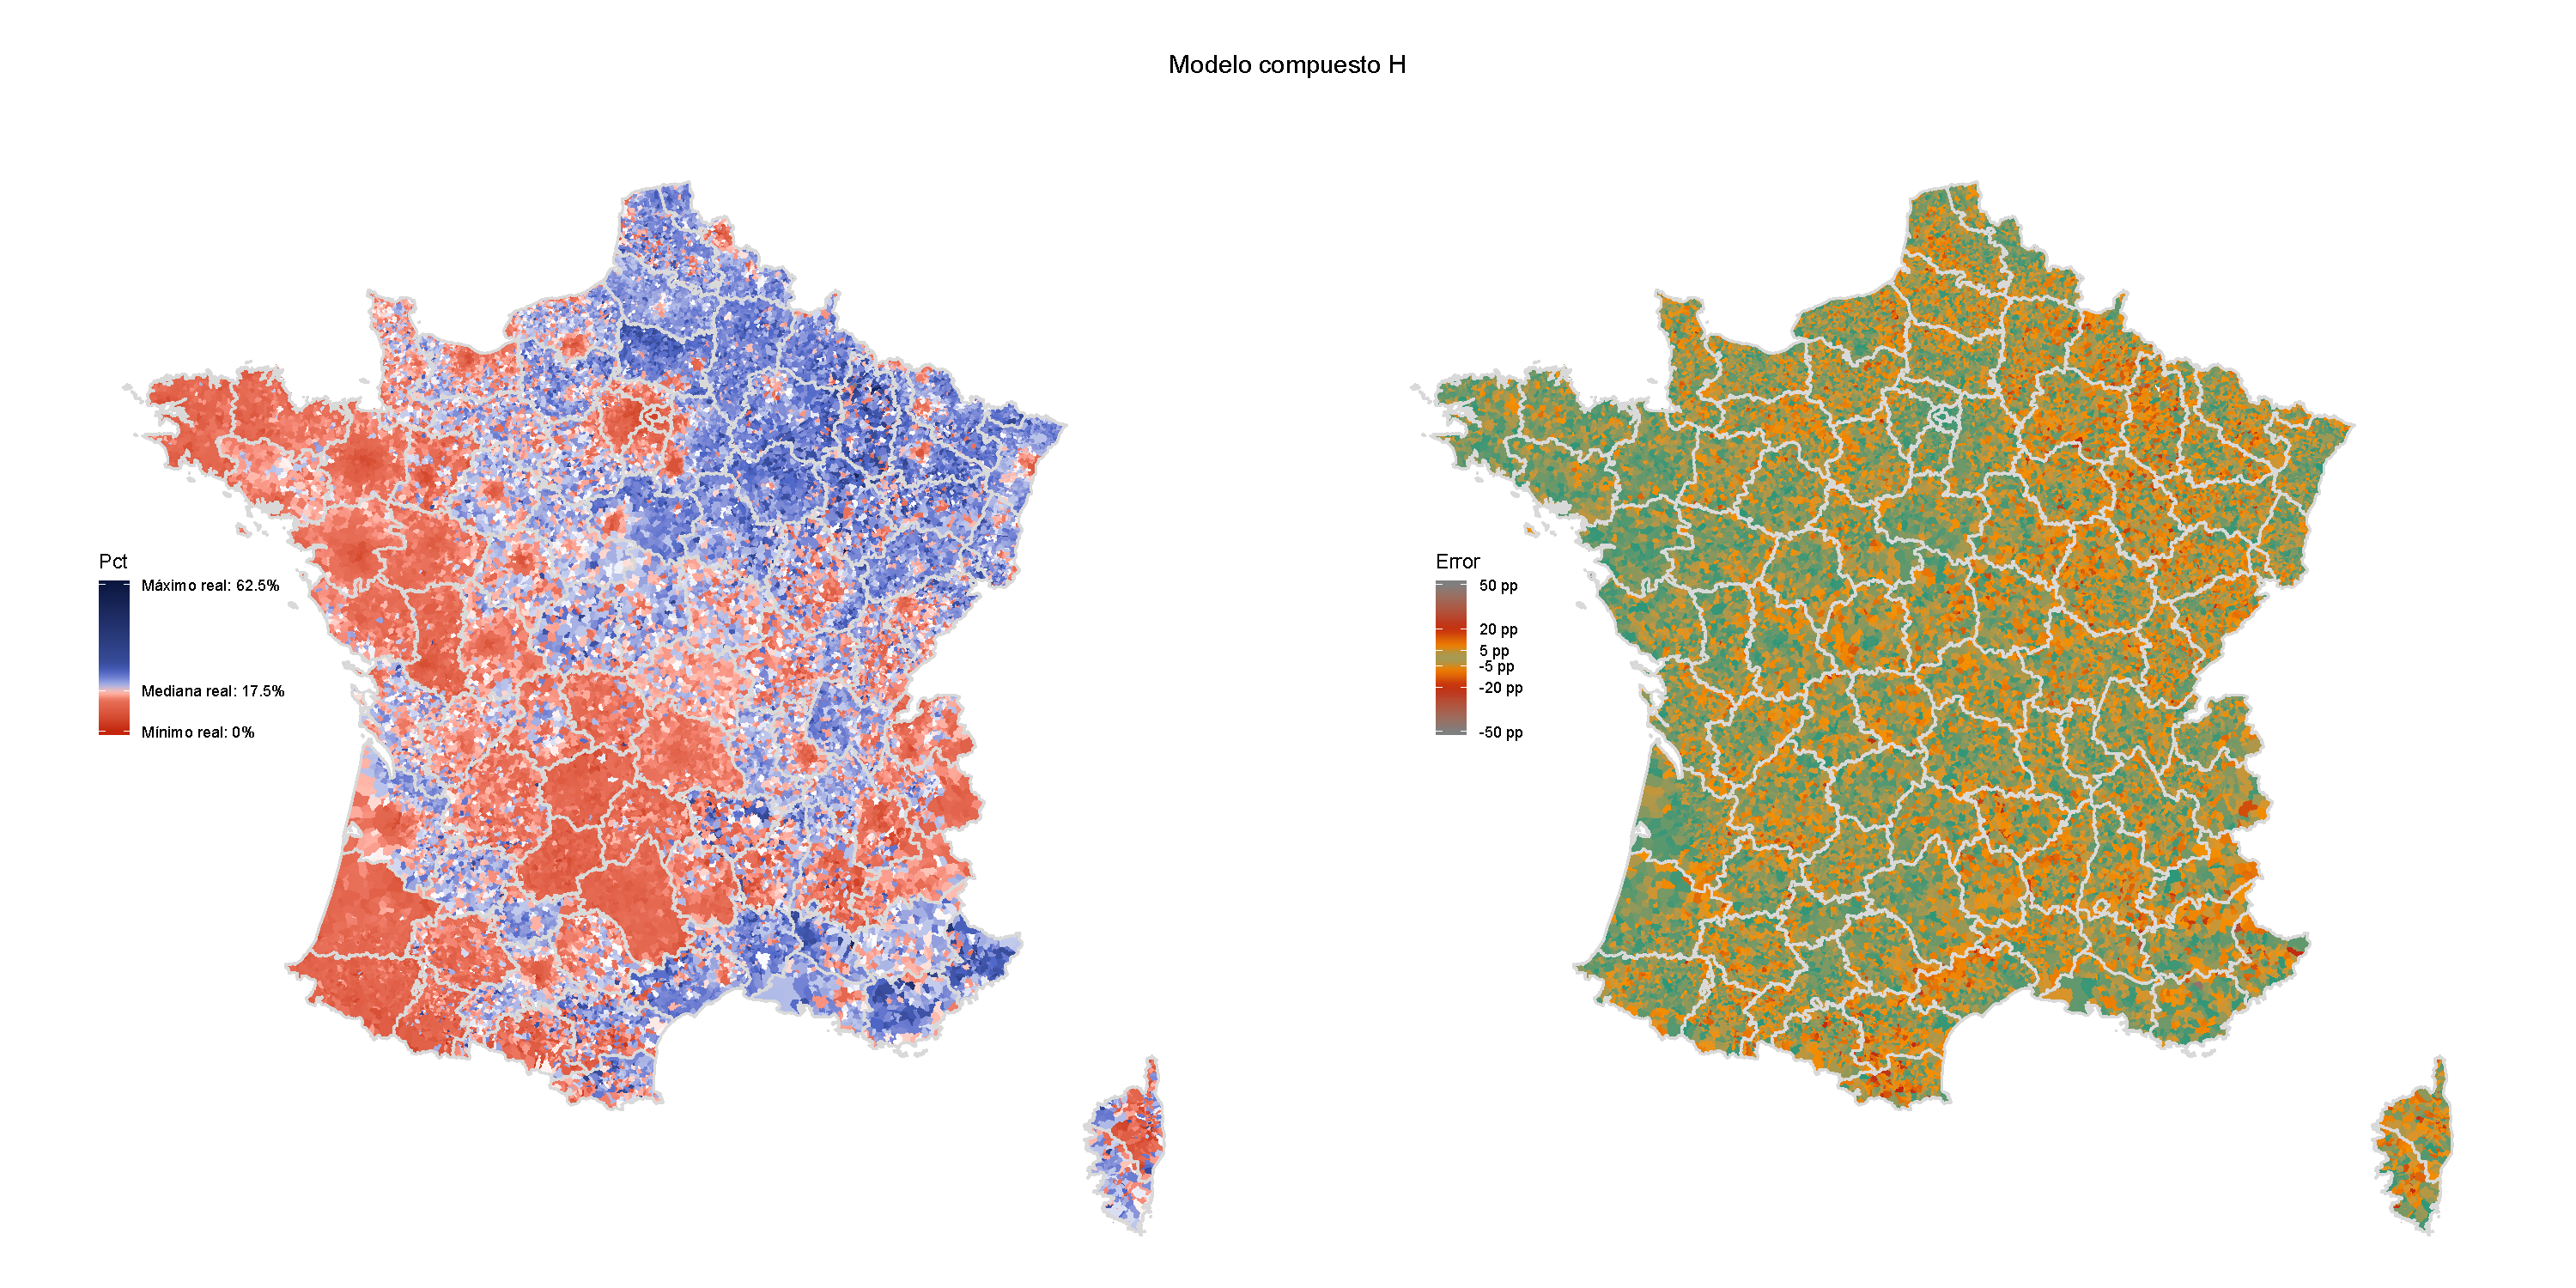
\includegraphics[width = 0.8\textwidth]{Figs/Modelado/Modelo_Compuesto_H}
	\caption{Mapas de predicciones medias (izq.) y respectivos errores (der.) para el porcentaje bruto de votos obtenido por Marine Le Pen en las presidenciales 2012 mediante el Modelo Jerárquico por Escolaridad, Categorías socioprofesionales, Edad, Condición migratoria, Sexo y Ocupaciones. Fuente: elaboración propia.}
	\label{fig:Modelo_Compuesto_H}
\end{figure}

En el mapa de la izquierda las predicciones se colorean de acuerdo a la escala real que va de 0\% a 62.5\% y donde el cambio de tonos rojos a azules se da en la comuna mediana de 17.5\%. Podemos compararlo con el verdadero mapa de resultados que observábamos en la \textbf{Figura \ref{fig:Mapa_Pct_Br}} del capítulo anterior. En la derecha vemos un mapa de errores en el que verde significa poco error y naranjas y rojos más. La mayor parte del hexágono se tiñe de verde por lo que podemos ver que el modelo tiene un buen ajuste predictivo a los datos reales.\\

Por otro lado, debo decir que interpretar los coeficientes de regresiones logísticas no es sencillo pues, por la función liga, estos se encuentran en una escala distinta a la de las proporciones o probabilidades que es en la que normalmente estamos interesados. Baste decir aquí que se realizaron los cálculos necesarios para poder interpretar los coeficientes de este modelo como el efecto predicho en puntos porcentuales al aumentar en 10 puntos porcentuales la proporción de individuos en la categoría de interés respecto a una comuna ``típica''. Tengo entonces la distribución posterior de los efectos con la que podemos continuar el análisis del modelo mediante distintos resúmenes inferenciales como el efecto mediano. Asimismo, podemos resumir la distribución reportando intervalos centrales de probabilidad al 95\% y, siguiendo la práctica común, cuando estos contengan al 0, diremos que la categoría poblacional no tiene un efecto significativo. Si, por el contrario, se encuentran en su totalidad por encima o por debajo del 0, diremos que se tiene un efecto significativo positivo o negativo, respectivamente.

\section{Escolaridad}

Comienzo el análisis de los efectos predichos por el modelo final por la variable de escolaridad, pues era la que los modelos individuales sugerían como más explicativa y sobre la que se fue construyendo el modelo 0 hasta llegar al H. En la \textbf{Figura \ref{fig:Mapa_Efectos_Escolaridad}} podemos observar el mapa de estimadores puntuales para los efectos departamentales por categorías de escolaridad bajo el modelo H. En cada departamento la intensidad de color refleja la magnitud del efecto mediano; en tonos rojos tenemos efectos negativos y en tonos azules efectos positivos.\\

\begin{sidewaysfigure}
	\centering
	\includegraphics[width = 0.9\textwidth]{Figs/Efectos/Mapa_Efectos_Escolaridad_Modelo_H}
	\caption{Estimaciones puntuales de los efectos de la escolaridad por departamento francés bajo el modelo H. Fuente: elaboración propia con la cartografía de Open Street Map.}
	\label{fig:Mapa_Efectos_Escolaridad}
\end{sidewaysfigure}

Inmediatamente observamos que la categoría universidad o más tiene un efecto negativo en prácticamente todo el hexágono francés. Algunos departamentos tienen magnitudes altas, reflejadas en la intensidad del color. Por el contrario, el aumento en el porcentaje de personas sin escolaridad parece llevar consigo un aumento en las preferencias por Marine Le Pen en la mayoría de departamentos. No obstante, vemos que en Córcega se daría el efecto contrario. En tonos más claros, es decir con una magnitud menor, el porcentaje de personas con escolaridad equivalente a la preparatoria parece también tener un efecto positivo en la afinidad por el FN. Los mapas de las personas que todavía están estudiando y de personas con primaria o secundaria parecen tener efectos mixtos, aunque los segundos se observan más intensos que los primeros.\\

Ahora bien, estos son solo estimadores puntuales. Una de las principales ventajas de los modelos jerárquicos bayesianos es que nos permiten reconocer la variabilidad de los fenómenos bajo estudio así como reportar la incertidumbre sobre ellos de manera más clara. En la \textbf{Figura \ref{fig:Efectos_Escolaridad}} tenemos un resumen de las distribuciones posteriores de los efectos. Para cada categoría observamos los 96 intervalos centrales de probabilidad al 95\% así como la mediana como estimador puntual que ordena los departamentos por categoría. Si el efecto se estima significativo--- es decir que el intervalo al 95\% excluye al 0---, observamos la distribución marcada en rosa o azul dependiendo del sentido de dicho efecto.\\

\begin{sidewaysfigure}
	\centering
	\includegraphics[width = 0.9\textwidth]{Figs/Efectos/Efectos_Escolaridad_Modelo_H}
	\caption{Intervalos centrales de probabilidad al 95\%, 80\% y 50\% para los efectos de la escolaridad por departamento francés bajo el modelo H. Los departamentos se ordenan para cada categoría por magnitud del estimador puntual que es el efecto mediano. Las distribuciones de colores rosa o azul representan que el efecto es significativo al 95\%. Las lineas verticales representan el efecto promedio a través de los departamentos. Fuente: elaboración propia.}
	\label{fig:Efectos_Escolaridad}
\end{sidewaysfigure}

Podemos hacer varias lecturas de este gráfico. En primer lugar confirmamos mediante las líneas verticales que, en general, un aumento en la proporción de personas con estudios universitarios disminuyó la afinidad comunal por Le Pen. De hecho, la mayoría de departamentos tienen efectos significativos; algunos, como Haute-Loire o Indre, incluso cercanos a -10 pp. ¡Esto es un efecto considerable, dado que estamos comparando una comuna promedio con una con 10 pp más de personas con escolaridad universitaria!\\

Por el contrario, el resto de categorías de escolaridad tienen efectos positivos en la afinidad frontista, aunque no todas en la misma magnitud y en todos los departamentos. Confirmamos que para las personas sin escolaridad la mayoría de departamentos tienen un efecto positivo, el más grande de al rededor de 5 puntos porcentuales por 10 de aumento en esta categoría poblacional. Pero también vemos que, aunque hay incertidumbre reflejada en la longitud del intervalo, en Haute-Corse el efecto es el contrario, aproximadamente de -1.8 pp.\\ 

La categoría de preparatoria tiene muchos departamentos con efectos significativos positivos y ninguno con efecto significativo negativo. Pero aquí también vemos al modelado jerárquico en acción. Aunque hayan muchos departamentos significativos, la incertidumbre es distinta a través de ellos. Comparemos por ejemplo las longitudes de los intervalos de los 7 departamentos con mayor efecto mediano. También podemos ver en el caso de las personas que todavía estudian que pueden existir efectos con un estimador puntual mayor al de otros, pero que no son significativos.\\

\begin{sidewaysfigure}
	\centering
	\includegraphics[width = 0.9\textwidth]{Figs/Efectos/Dorling_Efectos_Escolaridad_Modelo_H}
	\caption{Estimaciones puntuales de los efectos de la escolaridad por departamento francés bajo el modelo H, solo se colorean los efectos significativos. Fuente: elaboración propia.}
	\label{fig:Dorling_Efectos_Escolaridad}
\end{sidewaysfigure}

Tomando en cuenta entonces el carácter de significancia o no de un efecto, podemos modificar el mapa de la \textbf{Figura \ref{fig:Mapa_Efectos_Escolaridad}} y convertirlo en el dorling de la \textbf{Figura \ref{fig:Dorling_Efectos_Escolaridad}}. En este último, solo tienen color los departamentos con efecto significativo, aunque reporto los efectos esperados en todos los departamentos. Aquí identificamos que las únicas zonas donde el efecto de los universitarios no parece ser significativo es en departamentos más rurales como el llamado \textit{Massif Central}. Por el contrario, si en general el porcentaje de personas que todavía estudian no parecía ser tan importante, aquí observamos que sus efectos significativos se concentran en la región de Île de France. 

\section{Categorías socioprofesionales}

La segunda variable a considerar son las categorías socioprofesionales. Como indicaba en la revisión de literatura esta es probablemente la variable más utilizada en el estudio de la sociología electoral francesa. A pesar de ello, los mapas de la \textbf{Figura \ref{fig:Mapa_Efectos_Cat_Socioprof}} aparecen descolorados para la mayoría de categorías, indicando efectos muy pequeños. Resalta inmediatamente un departamento al noreste francés coloreado con un azul más intenso en el panel de obreros, la que es la categoría que parece tener una mayor asociación positiva con las preferencias por Marine Le Pen. Esto refuerza las hipótesis sobre \textit{gaucho-lépénisme} discutidas en la primera parte de este trabajo. Llama particularmente la atención la falta de intensidad en los efectos de los artesanos, comerciantes y empresarios, un grupo tradicionalmente asociado al FN. Otro punto interesante es notar que los cuadros y las profesiones intelectuales superiores tienen un efecto negativo, salvo en pocos departamentos que aparecen claramente en azul.\\ 

Al observar los intervalos de los efectos en la \textbf{Figura \ref{fig:Efectos_Cat_Socioprof}}, confirmamos que la mayoría de las categorías tienen efectos muy pequeños de acuerdo a los promedios a través de departamentos observados en las líneas verticales. La única categoría con un efecto promedio mayor parece ser la de los obreros donde Meuse es el departamento con el mayor efecto, de más de 4 puntos porcentuales. Esta también sería la categoría socioprofesional más cercana a un sentimiento de clase lo que podría explicar su mayor homogeneidad nacional frente a otras categorías que, como la investigación de \textcite{MayerMichelat81} ya sugería, pueden cambiar más sus inclinaciones políticas dependiendo del contexto local, reafirmando incluso la influencia que la mayor presencia de obreros tiene en la preferencia electoral de otras categorías.\\ 

Llama la atención también que para las profesiones intermediarias la mayoría de los efectos significativos son negativos, sin embargo tenemos 4 departamentos con claros efectos positivos y todos en zonas de fortaleza del FN: Vaucluse, Alpes-Maritimes y Hérault en el litoral mediterráneo y Aube en el noreste francés. El caso de los retirados es interesante porque si bien la mayoría de los efectos son nulos, hay algunos significativos tanto positivos como negativos y la gráfica se ve más dispersa.\\ 

Este es un ejemplo donde el modelo jerárquico se asemeja más a un modelo de no agregación o regresiones independientes. Por el contrario, las gráficas en la que las curvas son casi verticales, indicando efectos muy parecidos para todos los departamentos, serían casos más parecidos a los modelos de agregación completa o una sola regresión nacional.\\ 

\begin{figure}[H]
	\centering
	\includegraphics[width = \textwidth]{Figs/Efectos/Mapa_Efectos_Cat_Socioprof_Modelo_H}
	\caption{Estimaciones puntuales de los efectos de la categoría socioprofesional por departamento francés bajo el modelo H. Fuente: elaboración propia con la cartografía de Open Street Map.}
	\label{fig:Mapa_Efectos_Cat_Socioprof}
\end{figure}

\clearpage
\begin{sidewaysfigure}
	\centering
	\includegraphics[width = 0.9\textwidth]{Figs/Efectos/Efectos_Cat_Socioprof_Modelo_H}
	\caption{Intervalos centrales de probabilidad al 95\%, 80\% y 50\% para los efectos de la categoría socioprofesional por departamento francés bajo el modelo H. Los departamentos se ordenan para cada categoría por magnitud del estimador puntual que es el efecto mediano. Las distribuciones de colores rosa o azul representan que el efecto es significativo al 95\%. Las lineas verticales representan el efecto promedio a través de los departamentos. Fuente: elaboración propia.}
	\label{fig:Efectos_Cat_Socioprof}
\end{sidewaysfigure}
\clearpage

\begin{figure}[H]
	\centering
	\includegraphics[width = \textwidth]{Figs/Efectos/Dorling_Efectos_Cat_Socioprof_Modelo_H}
	\caption{Estimaciones puntuales de los efectos de la categoría socioprofesional por departamento francés bajo el modelo H, solo se colorean los efectos significativos. Fuente: elaboración propia.}
	\label{fig:Dorling_Efectos_Cat_Socioprof}
\end{figure}

La geografía de los efectos significativos que se observa en los dorlings de la \textbf{Figura \ref{fig:Dorling_Efectos_Cat_Socioprof}} tiene algunos puntos notables. El norte más industrializado se asocia con mayores efectos de la clase obrera. Vemos la particularidad del litoral mediterráneo en términos de profesiones intermediarias. Quizás sorprende que en París una mayor presencia de cuadros lleva a una mayor preferencia frontista. La explicación podría estar en que los cuadros que logran vivir dentro de París tiendan a ser más cercanos a la derecha, pero esta tendría que ser una hipótesis a explorarse con mayor detalle en otro tipo de estudio. 

\section{Edad}

Las explicaciones culturalistas, principalmente las de la escuela de Inglehart, hablan de que las generaciones de edad crecen con ciertos valores que los llevan a tener determinadas posiciones políticas. En este sentido podríamos leer los mapas de la \textbf{Figura \ref{fig:Mapa_Efectos_Edad}} como reflejo de los valores generacionales, lo que explicaría la mayor homogeneidad a través de departamentos frente a las variables antes analizadas. La mayor presencia de adultos mayores estaría relacionada negativamente con el FN porque este grupo de edad tiene una simpatía por la derecha tradicional. Los jóvenes de entre 18 a 24 años, por el contrario, tendrían posiciones políticas contrarias al carácter NAP del FN. La asociación positiva con los menores de edad podría reflejar un efecto cultural en comunas con altas tasas de natalidad o menos avejentadas. Esta hipótesis podría también explicar por qué los departamentos que parecen tener la tendencia contraria son aquelos de Île de France: la mayor presencia de inmigrantes, que normalmente tienen mayores tasas de natalidad, frenaría el voto nativista que los rechaza. Tendríamos que confirmar esto al analizar el efecto que los inmigrantes tuvieron según el modelo.\\

\clearpage
\begin{sidewaysfigure}
	\centering
	\includegraphics[width = 0.9\textwidth]{Figs/Efectos/Mapa_Efectos_Edad_Modelo_H}
	\caption{Estimaciones puntuales de los efectos del grupo de edad por departamento francés bajo el modelo H. Fuente: elaboración propia con la cartografía de Open Street Map.}
	\label{fig:Mapa_Efectos_Edad}
\end{sidewaysfigure}
\clearpage

\clearpage
\begin{sidewaysfigure}
	\centering
	\includegraphics[width = 0.9\textwidth]{Figs/Efectos/Efectos_Edad_Modelo_H}
	\caption{Intervalos centrales de probabilidad al 95\%, 80\% y 50\% para los efectos del grupo de edad por departamento francés bajo el modelo H. Los departamentos se ordenan para cada categoría por magnitud del estimador puntual que es el efecto mediano. Las distribuciones de colores rosa o azul representan que el efecto es significativo al 95\%. Las lineas verticales representan el efecto promedio a través de los departamentos. Fuente: elaboración propia.}
	\label{fig:Efectos_Edad}
\end{sidewaysfigure}
\clearpage

\clearpage
\begin{sidewaysfigure}
	\centering
	\includegraphics[width = 0.9\textwidth]{Figs/Efectos/Dorling_Efectos_Edad_Modelo_H}
	\caption{Estimaciones puntuales de los efectos del grupo de edad por departamento francés bajo el modelo H, solo se colorean los efectos significativos. Fuente: elaboración propia.}
	\label{fig:Dorling_Efectos_Edad}
\end{sidewaysfigure}
\clearpage

Al observar los resúmenes distribucionales confirmamos que los menores de edad y los adultos mayores son los grupos de edad que tienen mayor variabilidad e incertidumbre. En la \textbf{Figura \ref{fig:Efectos_Edad}} vemos que sus intervalos son claramente más largos que los del resto de categorías. De nueva cuenta, modelar mediante una estrategia multinivel tiene la ventaja de permitir que los datos determinen el nivel de agrupamiento necesario sin que el estadístico force a que deba ser total, con una sola regresión, o nulo via regresiones independientes. Observando los dorlings de la \textbf{Figura \ref{fig:Dorling_Efectos_Edad}} vemos que los efectos significativos negativos del grupo de 18 a 24 años se ubican tanto al oeste francés como en el norte. Por otro lado, los mayores de 65 años parecen tener una mayor influencia en el sur del hexágono.

\section{Categorías dicotómicas}

Finalmente, podemos analizar los mapas de las variables dicotómicas, es decir las que tienen solo dos categorías: Sexo, Condición migratoria y (des)ocupaciones. En la \textbf{Figura \ref{fig:Mapa_Efectos_Dicotom}} vemos que la mayor presencia de inmigrantes como de mujeres parece inhibir el voto frontista. Por el contrario, las variables de desempleo no reflejan una geografía muy clara pero sí con efectos en ambos sentidos. Al observar los intervalos de la \textbf{Figura \ref{fig:Efectos_Dicotom}} para estas categorías, nos damos cuenta que existe mucha incertidumbre en las estimaciones, salvo en la del desempleo juvenil. Esto parece continuar confirmándonos que esta no resulta ser la variable con mayor poder explicativo, al menos en términos de configuraciones sociales de las comunas.\\ 

\clearpage
\begin{sidewaysfigure}
	\centering
	\includegraphics[width = 0.9\textwidth]{Figs/Efectos/Mapa_Efectos_Dicotom_Modelo_H}
	\caption{Estimaciones puntuales de los efectos de categorías dicotómicas por departamento francés bajo el modelo H. Fuente: elaboración propia con la cartografía de Open Street Map.}
	\label{fig:Mapa_Efectos_Dicotom}
\end{sidewaysfigure}
\clearpage

\clearpage
\begin{sidewaysfigure}
	\centering
	\includegraphics[width = 0.9\textwidth]{Figs/Efectos/Efectos_Dicotom_Modelo_H}
	\caption{Intervalos centrales de probabilidad al 95\%, 80\% y 50\% para los efectos de categorías dicotómicas por departamento francés bajo el modelo H. Los departamentos se ordenan para cada categoría por magnitud del estimador puntual que es el efecto mediano. Las distribuciones de colores rosa o azul representan que el efecto es significativo al 95\%. Las lineas verticales representan el efecto promedio a través de los departamentos. Fuente: elaboración propia.}
	\label{fig:Efectos_Dicotom}
\end{sidewaysfigure}
\clearpage

\clearpage
\begin{sidewaysfigure}
	\centering
	\includegraphics[width = 0.9\textwidth]{Figs/Efectos/Dorling_Efectos_Dicotom_Modelo_H}
	\caption{Estimaciones puntuales de los efectos de categorías dicotómicas por departamento francés bajo el modelo H, solo se colorean los efectos significativos. Fuente: elaboración propia.}
	\label{fig:Dorling_Efectos_Dicotom}
\end{sidewaysfigure}
\clearpage

En el caso de la inmigración, las teorías del conflicto no parecen encontrar eco al observar los dorlings de la \textbf{Figura \ref{fig:Dorling_Efectos_Dicotom}}. Ciertamente aquí podríamos arriesgarnos a hablar de inferencia a nivel individual. Si una mayor proporción de inmigrantes adquieren derecho al voto, uno esperaría que no eligieran al partido NAP que resulta ser el FN. Por lo mismo, una mayor presencia de inmigrantes reduciría el voto frontista. Pero también existen las hipótesis que mencionan que el contacto con el inmigrante disminuye la xenofobia al comprobar que el otro no es tan diferente como se temía. En este sentido las explicaciones de un efecto indirecto de la presencia de inmigrantes parecerían más prometedoras que aquellas de xenofobia directa. Finalmente, para el caso de los desempleos observamos un claro contraste en la intensidad de los departamentos significativos entre el desempleo juvenil y el resto de categorías.\\ 

Con base en este análisis gráfico procederé en el siguiente capítulo a resumir las conclusiones del estudio así como algunas reflexiones sobre trabajo futuro y extensiones. 
	\chapter{Conclusiones}

Esta tesis aborda uno de los fenómenos políticos internacionales que, desde mi punto de vista, resulta por de más interesante de estudiar: los movimientos nativistas y autoritarios de corte populista que comúnmente son denominados con etiquetas como derechas radicales o extremas. Un buen punto de partida para estudiar estos movimientos es considerar uno de los partidos más característicos de esta corriente política, el \textit{Front National} francés. Utilizando datos oficiales del censo francés realicé un modelo estadístico de regresión que explicara el voto obtenido por el FN en las elecciones presidenciales del 2012 a partir de las distintas configuraciones sociales que dichos datos definen. Así, este modelo arroja varias lecciones.\\

En primer lugar, debo decir que el análisis estadístico refuerza lo que una parte importante de la literatura revisada sugiere. El clivaje de escolaridad es, probablemente, el más importante o explicativo a la hora de estudiar a estos movimientos NAP. Una mayor presencia a nivel local de personas con escolaridad universitaria o superior inhibió más el voto frontista en 2012 que cualquier otra de las variables consideradas. Por el contrario, una configuración social con mayor presencia de personas sin escolaridad formal o cuyo máximo grado de estudios fue la preparatoria favoreció el voto por la candidata del FN. Me resulta interesante que la variable de escolaridad sea, en este sentido, la más significativa pues es una variable que puede incorporar los dos \textit{resentimientos} que la literatura relacionaría con el fenómeno NAP: el cultural y el económico. La escolaridad tiene consecuencias económicas pero fundamentalmente puedo influir en los valores e ideas que tienen los individuos.\\

En este sentido, podemos conjeturar que ambas explicaciones coexisten pero parecería que la influencia de la ansiedad económica o la consciencia de clase es menor que aquella de la ``cultura política'' entendida como el conjunto de valores sociales e ideología que guía las decisiones políticas de los individuos. La variable socioeconómica por excelencia en los estudios de sociología electoral francesa que rescato de la literatura es la categoría socioprofesional de las personas. A pesar de contribuir a la explicación, parece que la única verdadera clase social--- en el sentido tradicionalmente entendido--- que favoreció el voto frontista fue la clase obrera, confirmando la existencia de un \textit{gaucho-lepensime}. Una mayor presencia de obreros estuvo asociada con un mayor voto frontista aunque en una magnitud menor que los efectos de las categorías de escolaridad. Por el contrario, una configuración social a nivel comuna con mayores niveles de cuadros y profesiones intelectuales inhibió el voto FN en 2012. ¿Existirá una consciencia de clase entre ellos o podemos pensar que el efecto se debe más a su asociación con contextos sociales culturalmente discordantes con el mensaje xenófobo y autoritario del FN?\\ 

Más aún, la influencia que tiene una distinta composición de la población comunal en términos de grupos de edades sería evidencia a favor de teorías culturalistas como las de Inglehart. Las comunas con mayores niveles de jóvenes entre 18 y 24 años tuvieron menor afinidad con Marine Le Pen en la elección presidencial. Las comunas más ``avejentadas'', en el sentido de contar con mayor presencia de personas retiradas o de más de 65 años, también votaron menos por Le Pen. Probablemente esto se deba a que la primera es una generación con valores y preocupaciones distintas a las del FN y, la segunda, la más cercana a la tradición gaullista de la derecha usual. En el sentido opuesto, las comunas con mayores porcentajes de menores de edad reflejaron mayor apoyo al FN. Esto ameritaría un estudio más detallado pero una primera hipótesis podría sugerir una sociedad más rural y también menos cercana a los valores posmodernos de familias pequeñas, mismos que podríamos asociar políticamente a partidos de izquierda como el socialista o el movimiento ecologista. En este mismo espíritu podríamos interpretar la mayoría de efectos negativos asociados a comunas con mayor presencia de mujeres.\\

Ahora bien, contrario a lo que la mayoría de las teorías sobre el conflicto o la competencia fiscal sugerirían que causa la presencia de inmigrantes, este estudio encuentra más bien una relación negativa con el voto frontista. Ello puede deberse a distintos factores. Una mayor cantidad de inmigrantes puede llevar a que más personas de este grupo accedan al derecho al voto, ya sea por naturalización o por un efecto de generaciones siguientes. Estos ciudadanos (pro)inmigrantes tenderían a rechazar el mensaje xenófobo de Le Pen. Adicionalmente, podría ser que la conviviencia a nivel local con inmigrantes elimine el miedo al \textit{Otro} que podría estar alimentando los sentimientos nativistas. Bajo esta hipótesis, más que un conflicto directo entre grupos estaríamos hablando de una xenofobia indirecta y de la ansiedad cultural que asocia la inmigración con un declive de las tradiciones europeas.\\

¿Es el desempleo reflejo de una descomposición económica que favorezca el surgimiento de los movimientos NAP? Hay referencias que particularmente señalan la ansiedad económica causada por el desempleo o fragilidad laboral juvenil. Esta tesis no parece encontrar que estas hipótesis sean las más favorecidas. De hecho, el desempleo juvenil podría considerarse como la variable menos explicativa de todas las aquí consideradas. Si bien observamos que el desempleo en general puede tener un efecto en el voto, este sería más modesto que otros y no en un mismo sentido a nivel nacioanl. En algunos lugares mayor desempleo favoreció el voto frontista y en otros lo inhibió.\\

Esta última consideración me lleva a llamar la atención sobre algo que parecería ser una respuesta frecuente en ciencias sociales y que en ocasiones pasamos por alto: depende. Muchas veces querríamos contar con teorías prístinas y unificantes como la existencia de ``El votante FN'' y sin embargo hay que recordar que la realidad es más compleja. Lo que los modelos de esta tesis señalan es que no existe una única relación entre las variables sociales consideradas. En este sentido estaríamos hablando de diferentes efectos dependiendo del contexto. La posibilidad de llevar a cabo un modelado jerárquico por departamento en lugar de conformarse con un modelo nacional más sencillo nos permite reconocer de mejor manera la variabilidad y la incertidumbre que tenemos sobre estos efectos. Mientras que hay variables con efectos más o menos homogéneos a nivel nacional, existen otras que influyen de manera marcadamente opuesta dependiendo del departamento del que hablemos.

\section*{Trabajo futuro}

Esta tesis, como es de esperarse, más que aportar respuestas definitivas genera nuevas preguntas tanto dentro del análisis de los movimientos NAP como respecto al contexto estadístico. Por lo mismo, señalo algunas de las posibilidades para continuar el estudio así como algunos comentarios respecto del proceso de modelado utilizado.\\

La primera forma de continuar el estudio de los movimientos NAP en general y el FN en particular es ajustar el modelo aquí desarrollado a otras elecciones. Están disponibles los datos para replicar el estudio en la elección del 2007 y, de acuerdo al calendario de difusión de resultados del INSEE, el próximo año contaremos con los datos censales necesarios para aplicarlos a la elección del 2017. El análisis de estas dos elecciones ofrecerían un panorama más completo de las configuraciones sociales del FN pues en la primera el candidato era Le Pen padre y no había pasado la crisis económica de 2008-2009 mientras que en la segunda Marine Le Pen accedió a la segunda vuelta presidencial lo que ofrece la posibilidad de estudiar ambas vueltas electorales. Podría verificarse qué factores han tenido continuidad y cuáles de las variables, de haberlas, han cambiado su efecto. Más aún, podrían también estudiarse las elecciones europeas y legislativas. Estas últimas, sin embargo, tienen la desventaja de no contar con la presencia de candidaturas frontistas en todos los lugares y ser elecciones que podríamos considerar como secundarias por lo que las motivaciones para votar por las diferentes fuerzas políticas suelen ser distintas.\\

Otra ruta es realizar un estudio de política comparada. Hoy por hoy, parecería que la batuta europea de los movimientos NAP la ha tomado la Lega de Matteo Salvini en Italia. El Istat, equivalente al INSEE francés o a nuestro INEGI, también ofrece datos que podrían permitir un estudio comparado de las configuraciones sociales de este partido italiano con aquellas del FN. Asimismo, pueden explorarse comparaciones con otros movimientos NAP. Finalmente, se podrían considerar otras variables además de las aquí utilizadas.\\

No quisiera terminar este trabajo sin reafirmar mi convicción de que la dignidad humana es sagrada. Por ello, busqué estudiar una corriente ideológica que, desde mi particular punto de vista, atenta constantemente contra ella. No es sino intentando entender por qué, cómo y dónde surgen estos movimientos que podremos dar respuestas y mitigar las consecuencias dañinas que de ellos se deriven. Es natural tener miedo por el futuro, pero deseo firmemente que quienes por distintas circunstancias lo experimenten, puedan encontrar esperanza sin odio a otros seres humanos. Pues, parafraseando al papa Francisco en su viaje a Mozambique, ningún país tiene futuro si el motor que une, convoca y tapa las diferencias de sus ciudadanos es el odio \parencite{Francisco}.
 
 



%%%%%%%%%%%%%%%%%%%%%%%%%%%%%%%%%%%%%%%%%%%%%%%%%%%%%%%%%%%%%
%%  REFERENCIAS %%%
%%%%%%%%%%%%%%%%%%%%%%%%%%%%%%%%%%%%%%%%%%%%%%%%%%%%%%%%%%%%%
\appendix

\addcontentsline{toc}{part}{Referencias}
\printbibliography[title = {Referencias}]

%%%%%%%%%%%%%%%%%%%%%%%%%%%%%%%%%%%%%%%%%%%%%%%%%%%%%%%%%%%%%
%%  FINAL DEL DOCUMENTO %%%
%%%%%%%%%%%%%%%%%%%%%%%%%%%%%%%%%%%%%%%%%%%%%%%%%%%%%%%%%%%%%

\end{document}